%
% Einfache LaTeX-Vorlage f�r Arbeiten am Lehrstuhl Kranzlm�ller / MNM-Team
% - optimiert f�r die Arbeit mit g�ngigen LaTeX-Editoren
% - funktioniert ohne Makefile und Anpassungen der LaTeX-Verzeichnisstruktur
% - verwendet Komaskript f�r ein (nach europ�ischen Gepflogenheiten) sch�neres Layout
% 
% v1, 2007 (Michael Brenner)
% v1.1, 2012 (Michael Brenner)
% v1.2, 2017 (Michael Brenner)
% Diese Version: v1.2.1, 2017 (Benjamin Schnoy)


\documentclass[bibliography=totoc,listof=totoc,BCOR=5mm,DIV=12]{scrbook} % Rand f�r Bindung: 5mm / falls Index verwendet, erg�nze "index=totoc" zu den Optionen 
\usepackage{ngerman} % Trennung nach neuer deutscher Rechtschreibung, deutsche Sonderzeichen, z.B. \glqq und \grqq f�r deutsche Anf�hrungszeichen 
\usepackage[latin1]{inputenc} % Umlaute im Text
\usepackage{graphicx} % Einf�gen von Grafiken  - f�r PDF-Latex: .pdf und .png (.jpg m�glich, sollte aber vermieden werden)
\usepackage{url}           % URL's (z.B. in Literatur) sch�ner formatieren
\usepackage{hyperref} % sorgt f�r f�r Hyperlinks in PDF-Dokumenten

\graphicspath{{./Bilder/}}

%
% der Befehl \hypenation versteht keine Sonderzeichen, also weder �
% noch "a noch \"a. W�rter die derartige Zeichen enthalten m�ssen
% direkt im Text getrennt werden, z.B. W�r\-ter
%
\hyphenation{Ma-nage-ment}
\hyphenation{Ma-nage-ment-agent}
\hyphenation{Ma-nage-ment-agent-en}
\hyphenation{Ma-nage-ment-ar-chi-tek-tur}
\hyphenation{Ma-nage-ment-ar-chi-tek-tu-ren}
\hyphenation{Ma-nage-ment-an-wen-dung}
\hyphenation{Ma-nage-ment-an-wen-dung-en}
\hyphenation{Ma-nage-ment-an-for-der-ung}
\hyphenation{Ma-nage-ment-funk-ti-on}
\hyphenation{Ma-nage-ment-funk-ti-onen}
\hyphenation{Ma-nage-ment-kon-zep-te}
\hyphenation{Ma-nage-ment-res-source}
\hyphenation{Ma-nage-ment-in-for-ma-ti-on}
\hyphenation{Ma-nage-ment-res-sour-cen}
\hyphenation{ma-nage-ment-re-le-vante}
\hyphenation{ma-nage-ment-sy-stem}
\hyphenation{ma-nage-ment-sy-steme}
\hyphenation{Ma-nage-ment-in-stru-men-tie-rung}
\hyphenation{Ma-nage-ment-platt-form}
\hyphenation{Sys-te-men}
\hyphenation{Sys-tem-um-ge-bun-gen}
\hyphenation{Sys-tem-ma-nage-ment}
\hyphenation{DHCP}
\hyphenation{Ma-nage-ment-diszi-plinen}
\hyphenation{System-management-architekturen}
\hyphenation{Verwendungs-nachweise}
\hyphenation{Video-einricht-ungen}
\hyphenation{Res-source}
\hyphenation{Res-sourcen}
\hyphenation{Grund-anwendung}
\hyphenation{Grund-anwendungen}
\hyphenation{Basis-anwendung}
\hyphenation{Core}
\hyphenation{Kom-mu-ni-ka-ti-on}
\hyphenation{De-sign-ent-schei-dung}
\hyphenation{Sprung-ad-res-sen}
\hyphenation{Klas-si-fi-ka-ti-on}
\hyphenation{Schreib-recht}
\hyphenation{Be-nut-zer-zer-ti-fi-kat}
\hyphenation{Bau-stein-ent-wi-ckler}
\hyphenation{ad-mi-ni-stra-ti-ve}

 % in dieses File kommen W�rter die Latex nicht richtig trennt

\begin{document}

% ---------------------------------------------------------------
\frontmatter % Titelbl�tter und Erkl�rung jeweils spezifisch f�r die jeweilige Uni einbinden
    %%%%%%%%%%%%%%%%%%%%%%%%%%%%%%%
% erste Seite

\thispagestyle{empty}

\begin{center}

\vspace*{-2cm}

{\Huge INSTITUT F�R INFORMATIK\\[1mm]}
DER LUDWIG--MAXIMILIANS--UNIVERSIT�T M�NCHEN\\

\vspace*{1cm}


\includegraphics[width=0.3\textwidth]{lmu_siegel}

\vspace*{2cm}

{\Large \textbf{Masterarbeit}}\\ % oder Fortgeschrittenenpraktikum, Master's Thesis, Bachelorarbeit etc.

\vspace{2.0cm}
{\Huge \textbf{Lorem Ipsum Dolor}}\\
\vspace*{3mm}
{\Huge \textbf{Sit Amet}}\\
\vspace*{3mm}
{\Huge \textbf{-- Adipiscing Elit}}\\
\vspace{1.5cm}

{\LARGE Vorname Nachname} % Name des Autors

\vspace{3cm}
Draft vom \today % erleichtert den Betreuern die Zuordnung - f�r finale Version entfernen

\end{center}

\newpage

%%%%%%%%%%%%%%%%%%%%%%%%%%%%%%%
% zweite Seite

\thispagestyle{empty}
\cleardoublepage

%%%%%%%%%%%%%%%%%%%%%%%%%%%%%%%
% dritte Seite (Kopie der ersten)

\thispagestyle{empty}

\begin{center}

\vspace*{-2cm}

{\Huge INSTITUT F�R INFORMATIK\\[1mm]}
DER LUDWIG--MAXIMILIANS--UNIVERSIT�T M�NCHEN\\

\vspace*{1cm}


\includegraphics[width=0.3\textwidth]{lmu_siegel}

\vspace*{2cm}

{\Large \textbf{Diplomarbeit}}\\ % oder Fortgeschrittenenpraktikum, SEP etc.

\vspace{2.0cm}
{\Huge \textbf{Lorem Ipsum Dolor}}\\
\vspace*{3mm}
{\Huge \textbf{Sit Amet}}\\
\vspace*{3mm}
{\Huge \textbf{-- Adipiscing Elit}}\\

\vspace{1.5cm}

{\LARGE Vorname Nachname} % Name des Autors
\vspace{2cm}

\parbox{1cm}{
\begin{large}
\begin{tabbing}
Aufgabensteller: \hspace{.5cm} \=Prof. Dr. Dieter Kranzlm�ller\\[2mm]
Betreuer:
\>MNM-Team-Betreuer 1\\ % alphabetische Reihenfolge (Nachname)
\>MNM-Team-Betreuer 2\\
\>Externer Betreuer 1 (Firma)\\[5mm]
Abgabetermin: \> 7. Juli 2077\\
\end{tabbing}
\end{large}}\\
\vspace{5mm}

\end{center}
 % Titelbl�tter LMU - auskommentieren falls TUM-Arbeit
%    % Richtlinien, siehe http://wwwpa.in.tum.de/generell/Abschlussarbeitsform.html
%
%%%%%%%%%%%%%%%%%%%%%%%%%%%%%%%


% Deckblatt

\thispagestyle{empty}

\begin{center}
    
\includegraphics[width=3cm]{tum-logo}\\
    \vspace{.5cm}
% "Technische Universit�t M�nchen" oder alternativ das Logo der TUM
    {\Large \textsc{Technische Universit�t M�nchen}}\\

    \vspace{1cm}
% "Fakult�t f�r Informatik"
    {\Huge \textsc{Fakult�t f�r Informatik}\\[1mm]}


    \vspace{2cm}
% Diplomarbeit | Master's Thesis | Bachelorarbeit in Informatik | Wirtschaftsinformatik |
    {\Large \textbf{Masterarbeit in Informatik}}\\
% Thema bzw. Titel der Arbeit  (In der Sprache, in der die Arbeit verfasst wurde)
    \vspace{2.0cm}
    {\Huge \textbf{Ein Lorem-Rahmenwerk}}\\ % bei langen Titeln ggf. Schriftgr��e auf \huge herunter setzen
    \vspace*{3mm}
    {\Huge \textbf{f�r Ipsum-Systeme}}\\
    \vspace*{3mm}
    {\Huge \textbf{-- ein Dolor-Ansatz}}\\
    \vspace{1.5cm}
% Vorname und Nachname des Bearbeiters/ der Bearbeiterin
    Vorname Nachname

    \vspace{5cm} % ggf. je nach Zeilenzahl und Schriftgr��e des Titels anpassen
    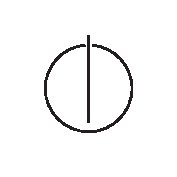
\includegraphics[width=2.4cm]{tum-info-logo}
\end{center}

\newpage

%%%%%%%%%%%%%%%%%%%%%%%%%%%%%%%
% R�ckseite Deckblatt

\thispagestyle{empty}
\cleardoublepage

%%%%%%%%%%%%%%%%%%%%%%%%%%%%%%%
% Erste Seite (Titelblatt)

\thispagestyle{empty}

\begin{center}

    
\includegraphics[width=3cm]{tum-logo}\\
    \vspace{.5cm}
    {\Large \textsc{Technische Universit�t M�nchen}}\\


    \vspace{.5cm}

    {\huge \textsc{Fakult�t f�r Informatik}\\[1mm]}


    \vspace{1cm}

    {\Large \textbf{Diplomarbeit in Informatik}}\\ % oder SEP etc.

% Thema bzw. Titel der Arbeit  (In der Sprache, in der die Arbeit verfasst wurde)
    \vspace{1.5cm}
    {\huge \textbf{Ein Lorem-Rahmenwerk}}\\ % bei langen Titeln ggf. Schriftgr��e herunter setzen
    \vspace*{3mm}
    {\huge \textbf{f�r Ipsum-Systeme}}\\
    \vspace*{3mm}
    {\huge \textbf{-- ein Dolor-Ansatz}}\\

% die englische bzw. deutsche Entsprechung des Titels
    \vspace{1cm}
    {\huge \textbf{A Lorem Framework}}\\ % bei langen Titeln ggf. Schriftgr��e herunter setzen
    \vspace*{3mm}
    {\huge \textbf{for Ipsum Systems}}\\
    \vspace*{3mm}
    {\huge \textbf{-- a Dolor Approach}}\\
    \vspace{1cm}

    \parbox{1cm}{
      \begin{large}
        \begin{tabbing}
          Bearbeiter: \hspace{1.5cm}
            \=Vorname Nachname\\[2mm]
    Aufgabensteller: \>Prof. Dr. Dieter Kranzlm�ller\\[2mm]
    Betreuer: \>MNM-Team-Betreuer 1\\ % alphabetische Reihenfolge (Nachname)
    \>MNM-Team-Betreuer 2\\
    \>Externer Betreuer 1 (Firma)\\[5mm]
    Abgabedatum: \> 7. Juli 2077\\
        \end{tabbing}
      \end{large}
    }\\

    \vspace{.3cm}

    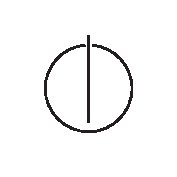
\includegraphics[width=2.4cm]{tum-info-logo}

\end{center}
 % Titelbl�tter TUM - auskommentiert lassen falls LMU-Arbeit
    \thispagestyle{empty}
    \cleardoublepage
    %
% LaTeX-Rahmen für Arbeiten am Lehrstuhl Hegering
%
% Harald Roelle, 2001, 2002
%
% basierend auf Arbeiten von Helmut Reiser, Boris Gruschke und Stephen Heilbronner
%

\newpage

\thispagestyle{empty}

\begin{large}

\vspace*{2cm}

\noindent
Hiermit versichere ich, dass ich die vorliegende Masterarbeit
selbständig verfasst und keine anderen als die angegebenen Quellen
und Hilfsmittel verwendet habe.

\vspace{2cm}

\noindent
München, den 19. Januar 2021

\vspace{3cm}

\hspace*{7cm}%
\dotfill\\
\hspace*{8.5cm}%
\textit{(Unterschrift des Kandidaten)}

\end{large}
 % Erkl�rung (Arbeit selbstst�ndig verfasst) - auskommentieren falls TUM-Arbeit
%    \begin{large}

\vspace*{2cm}
\noindent
Ich versichere, dass ich diese Masterarbeit % (bzw. Master's Thesis)
selbst�ndig verfasst und nur die angegebenen Quellen und Hilfsmittel verwendet habe.

\vspace{2cm}

\noindent
M�nchen, den 7. Juli 2077

\vspace{3cm}

\hspace*{7cm}%
\dotfill\\
\hspace*{8.5cm}%
\textit{(Unterschrift des Kandidaten)}

\end{large}
 % Erkl�rung (Arbeit selbstst�ndig verfasst) - auskommentiert lassen falls LMU-Arbeit
    \thispagestyle{empty}
    \cleardoublepage
    \vspace*{2cm}

\begin{center}
    \textbf{Abstract}
\end{center}

\vspace*{1cm}

\noindent In the last 40 years, quantum computing developed from an exclusively theoretical description of a quantum Turing machine to real-world implementations with various technologies and capabilities. Linking this development to digital computer's rapid development in the 20th century, a quantum computer with practical implications on industry and everyone's daily life seems within reachable bounds. There are many reasons to seek such a practical implementation. From algorithmic improvements to completely new technical possibilities like quantum teleportation, a quantum computer promises to solve certain tasks faster than possible with a classical digital computer.

\par Besides the benefits such a computer could provide, it would also have a significant impact on cryptography. Modern cryptography protocols in general and especially the field of public-key cryptography relies on mathematical problems that are believed to be intractable. Famous examples of such algorithms are the RSA and the Diffie-Hellman (DH) key exchange protocol and its variant, Elliptic Curve Diffie-Hellman (ECDH). Today, nearly all encrypted messages in the modern Web are bootstrapped by either one of these protocols. A serious flaw in these cryptosystems would have a massive impact on the confidentiality of user data. This is where quantum computing comes into play. In 1999 Peter Shor published his famous algorithm, which uses a quantum computer to break both the RSA and the DH problem. Since Shor was able to show that both algorithms run in polynomial time, the foundation of modern cryptography is questioned.

Luckily, even more than 20 years later, there is no implementation of a quantum computer available that could be used to break cryptographic keys of reasonable size. While this may not be true in the more distant future, an ever-growing effort was introduced to find alternative, quantum-safe cryptosystems for which no such attack exists.

This work focuses on the adaptation and evaluation of such algorithms for IEEE 802.1X and IEEE 802.1AE. IEEE 802.1X focuses on the mutual authentication of clients in IEEE 802.1 Ethernet networks. For this purpose, asynchronous digital signature schemes are used that are directly affected by Shor's algorithm. Furthermore, 802.1X uses public-key cryptography and key exchanges to agree on a symmetric key between the clients and the connected network equipment. This work provides a design for a quantum-safe implementation of EAP-TLS, which can be used in IEEE 802.1X to mitigate attacks that involve a quantum computer. An extensive evaluation of the performance of different signature and key exchange algorithms is provided, and as a proof-of-concept, a real-world implementation is benchmarked with selected post-quantum and classical algorithms. % Abstract
    \thispagestyle{empty}
    \tableofcontents % Inhaltsverzeichnis

% ---------------------------------------------------------------
\mainmatter % die eigentliche Arbeit

    \chapter{Introduction}

Quantum Computing is a promising field of research for computer scientists. In this context, the term ``quantum'' refers to the mathematical description of the physical phenomena of quantum mechanics as described in the 20th century by researchers like Werner Heisenberg, Erwin Schrödinger, Paul Dirac and John von Neumann. Quantum mechanics provide a mathematical framework that tries to cope with problems in the so-called classical physics theory, which turns out to have problems explaining phenomena on atomical scales. One of the first researchers who recognized the implications of the quantum mechanical approach on computer science was physicist Paul Benioff. In his paper, he described a ``microscopic quantum mechanical model of computers as represented by Turing machines''\cite{benioff1980computer}. Since the first description of such a computer, multiple approaches for quantum-aware computing machines were proposed. Two major contributions to this field are the so-called Adiabatic Quantum Computing and the \ac{QGM}. This thesis focuses on the implications of Shor's and Grover's algorithm on modern cryptography. Both algorithms are derived from the \ac{QGM} and weaken or even break important guarantees of commonly used cryptographic protocols. In the remainder of this thesis, these implications for the MACSec protocol suite are highlighted, and alternatives for a quantum-resistant variant are discussed and evaluated.

\section{Motivation}
The \ac{QGM} provides a mathematical description of a theoretical approach to build a quantum computer. This model uses qubits and logical ``quantum gates'' in analogy to bits and logical gates as used in classical computing theory. A single qubit is a two-dimensional vector that represents the state of this qubit. It is possible to transform a qubit's state by applying logical gates, represented by unitary matrices. Applying a logical gate is equivalent to ordinary matrix-vector multiplication of the qubit vector with the corresponding gate matrices. An algorithm in the \ac{QGM} consists of several qubits and a set of unitary matrices applied in a particular order. One of the first algorithms with a so-called quantum advantage over a classical algorithm was described by David Deutsch and Richard Josza and hence is often called the Deutsch-Josza algorithm. This algorithm computes whether a function \(f : \{0,1\}^n \rightarrow \{0, 1 \} \) is balanced or constant in a single iteration on a theoretical quantum computer\cite{deutsch1992rapid}. While this algorithm has mostly theoretical relevance to the field, different algorithms with a more practical approach were proposed in the last years. The Deutsch-Josza algorithm shows an essential property of practical quantum computers: Problems that are regarded as computationally too hard to solve on a classical computer may be solved efficiently by a quantum computer. One example of such a problem is the factorization of the product of two large prime numbers, which belongs to the complexity class NP and for which no polynomial-time solving algorithm is known. This specific problem was used to construct the RSA cryptosystem, developed by Rivest, Shamir and Adleman in 1978\cite{rivest1978method}. RSA is one of the most important and widely used cryptographic primitives in modern cryptographic protocols, and its secureness critically relies on the complexity of this problem. In 1999, Peter Shor proposed an algorithm for a quantum computer, built on the foundations of the quantum gate model, that factorizes large numbers in polynomial time on a quantum computer, using an implementation of the fast Fourier transformation. Shor even speculated that the quantum Fourier transformation could be used to speed up multiplication itself, resulting in lower asymptotical bounds for the time needed to break RSA on a quantum computer than performing the encryption on a classical computer.

Furthermore, Shor shows in his work how to apply the proposed quantum Fourier transformation to calculate the discrete logarithm \(x\) of a number \(m = g^x \bmod p\) in polynomial time. This variant can be used to break the security of the widely used discrete \ac{DH} public-key exchange and its variant \ac{ECDH}\cite{shor1999polynomial}. \ac{DH}-based protocols have gained significant importance in the last years and even superseded RSA-based key exchanges in many cases. An example is the widely used TLS protocol, which in its recent 1.3 version completely dropped support for RSA-based key exchanges in favor of \ac{DH} and \ac{ECDH}-based approaches.

\begin{figure}[ht]
    \centering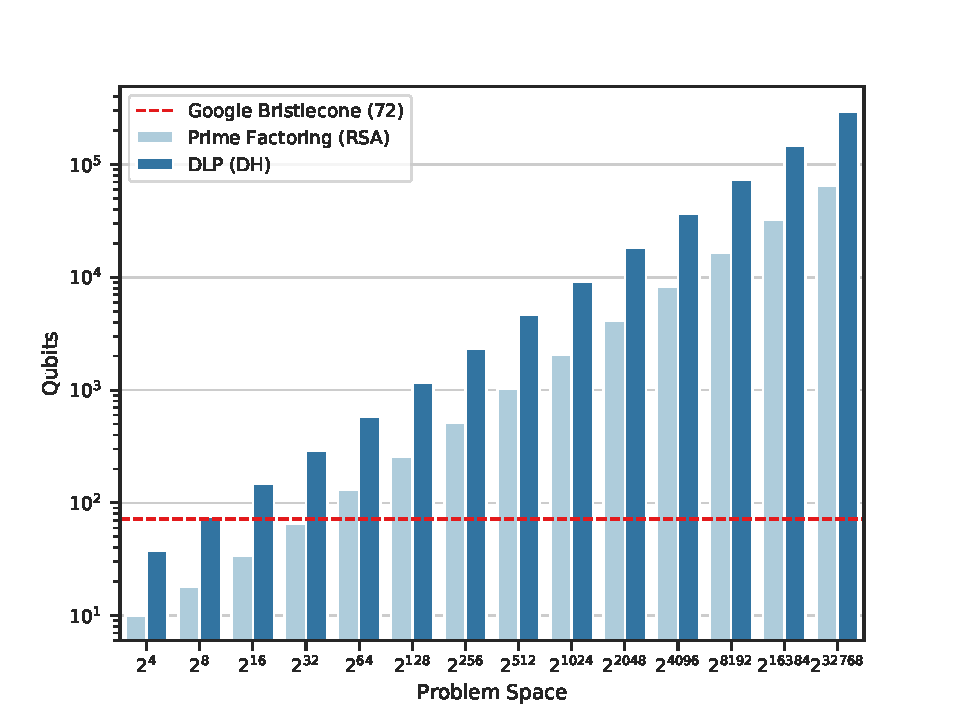
\includegraphics[width=1.0\linewidth]{plot_line_shor_rsa.pdf}
    \caption{Estimates of the number of qubits needed to break an RSA/ECC problem of a certain size. The y-axis is logarithmic to a base of two. The estimated number for breaking an RSA key of \(2^n\) is \(2n+2\), according to \cite{haner2017factoring}. For an ECC \ac{DLP} of size \(2^n\) the number is \(9n+2\ln(n)\), according to \cite{roetteler2017quantum}. The dotted, red line shows the amount of currently available physical qubits supported by Google's Bristlecone architecture (\(72\)).}\label{fig:shor_vs_rsa_dlog}
\end{figure}


Lov Grover proposed another important algorithm in 1996\cite{grover1996fast}. Grover described a quantum mechanical algorithm for searching a key in an unsorted database with \(n \) elements. The proposed algorithm has a runtime of \(\bigo(\sqrt{n})\) as opposed to a classical algorithm that needs to take \(\bigo(n)\) steps, given the number of elements. This algorithm is also of particular interest to the cryptographic community since the best-known approach for many symmetrical cryptosystems is a brute force attack, which can be reduced on a random search in the keyspace of the symmetrical cipher. For symmetrical keys with size \(2^n \), the search space is therefore effectively halved by Grover's algorithm.

Both algorithms were already implemented in real-world experimental setups. In 2001 Vandersypen et al. factored the number 15 by implementing Shor’s algorithm on a quantum computer\cite{vandersypen2001experimental}. Due to limitations in the practical realization of sufficient large quantum computers, as of today, there is no realistic scenario where Shor's algorithm can be used to break state-of-the-art encryption in the next decade. Figure~\ref{fig:shor_vs_rsa_dlog} shows an overview of how many qubits are needed to break a cryptosystem of a specific size alongside the number of available qubits on Google's Bristlecone Architecture, one of the largest quantum computer implementations available today. The number of needed and available qubits are specified as ``physical'' qubits, meaning that the number of available qubits on a single quantum computer may be smaller, while the number of needed ``logical'' qubits to break a particular key may be magnitudes of order higher. The main reason is the need for error correction. Even in the optimistic scenario with no need for error correction, as of today, no available quantum computer is close to breaking any encryption scheme with a reasonable key size. However, in the last years, an ever-growing effort was put into building a more capable quantum computer. While it is difficult to compare such systems directly, a standard measure is the number of coherent qubits realized. In cooperation with Oak Ridge National Laboratory and Google, the \ac{NASA} was recently able to show so-called ``quantum supremacy'' or ``quantum advantage'' on a quantum computer design that uses 54 qubits\cite{arute2019quantum}. While this number and other properties like coherence time on these machines may be magnitudes of orders too small for a practical application, an exponential development of these parameters, similar to Moore's law, must be assumed. The issue gets even more pressing when considering that governmental agencies may already be storing large amounts of encrypted data in specially tailored data centers for later decryption.\footurl{https://www.wired.com/2012/03/ff-nsadatacenter/} This renders currently used cryptographic systems unusable for future applications and raises the need for two important tasks: Finding new algorithms that rely on different problems and provide better resistance against attackers with access to a sufficiently large quantum computer and second, identify currently used protocols and system which rely on cryptographic protocols that are known to be vulnerable against such attackers and securing them against quantum-adversary.

One class of protocols heavily used to encrypt and authenticate data streams are so-called \ac{VPN} protocols. \acp{VPN} are commonly used to span a virtual, encrypted network link between two, often geographically separated networks. These connections are virtual in the sense that for the computing equipment in such networks, it looks like they reside in the same \ac{LAN} while the network traffic is transmitted over different public network links. Encryption schemes are used in such protocols to keep the transmitted data confidential, even during transmission over untrusted lines. Solutions like IPSEC\cite{rfc4301}, OpenVPN\footurl{https://openvpn.net/} and Wireguard\footurl{https://www.wireguard.com/} are commonly used to connect IP-Layer network links, while protocols like MACSec as defined by IEEE 802.1AE\cite{IEEE8021AE} are used to connect two nodes in the same \ac{LAN} directly. MACSec is often used in places like carrier-grade interconnects where control over the physical link itself may not be possible. Due to the amount of data usually transmitted over such links and the broad number of subscribers, a single carrier can be the bottleneck for data and, as such, can be of particular interest to an attacker. This may be even further relevant in the context of \ac{PQ} security when taking into account that the first sufficient large quantum computers are probably going to be owned by large organizations, which are likely also have the resources to access such network interconnects directly.

\section{Problem Statement}
This thesis is part of the QuaSiModO project\footurl{https://www.pq-vpn.de/index.html} and focuses on the 802.1X and 802.1AE protocol suites provided by the \ac{IEEE}. Cryptographic schemes are an essential part of this wieldy employed protocol suite, used for authentication and encryption in wired, as well as in wireless networks. This thesis aims to identify used cryptographic protocols and an evaluation of their vulnerability to attackers with a (theoretical) sufficient large quantum computer. Currently, a broad range of post-quantum algorithms is available. It is crucial to not only select an arbitrary alternative but to evaluate their performance regarding the protocol's design goals and select a candidate, which allows for a future proof design that can be used as a drop-in replacement. Optimally, a replacement should ensure security against quantum adversaries and additionally keep into account that computing resources may be constrained.

\section{Methodology}
In Chapter~2, an overview of the details of the used technologies and protocols is provided. It covers the \ac{IEEE} 802.1X and 802.1AE protocol suites and provides an overview of quantum computing with a particular focus on \ac{PQC}. Furthermore, an overview of work related to this field is provided. Chapter 3 defines requirements for a PQ implementation of the 802.1X protocol suite, depending on used cryptographic algorithms in 802.1X and limitations from the used Ethernet layer. The fourth chapter focuses on a design proposal of a quantum-resistant implementation of the 802.1X protocol. Available alternatives to the used cryptographic schemes shall be evaluated, and a proposal to harden the protocol suite shall be provided. This thesis does explicitly not aim to employ new quantum-resistant cryptographic schemes but rather evaluates existing schemes and selects them to fit the requirements that arise from the characteristics of the concerned protocols. The selection of the cryptographic protocols is tightly coupled to an ongoing project, hosted by the \ac{NIST}, that aims to ``solicit, evaluate, and standardize one or more quantum-resistant public-key cryptographic algorithms''\footurl{https://csrc.nist.gov/projects/post-quantum-cryptography}. Vulnerable components of the protocol are outlined, and appropriate countermeasures are provided. The fifth chapter focuses on an experimental evaluation of the proposed design.

\endinput
%    \chapter{Background}

This chapter provides an overview of the used technologies. The first section describes the IEEE 802.1X protocol suite in version 802.1X-2010 and the IEEE 802.1AE protocol suite in the version 802.1AE-2018. The second section focuses on the field of \ac{PQC}. It provides an overview of the ongoing \ac{NIST} standardization project, emphasizing the mathematical background of the used key exchange and signature algorithms. Further, common limitations and trade-offs specific to these algorithms are discussed. In the last part of this chapter, an overview of related research concerning applications for post-quantum cryptosystems in general and 802.1X and 802.1AE, in particular, is provided.

\section{IEEE 802.1X}
The primary purpose of the 802.1X protocol suite is the mutual authentication of clients and network equipment in wired and wireless \ac{LAN} networks, as well as the establishment of so-called \ac{SA} used by the IEEE 802.1AE MAC Security standard\cite{IEEE8021X}. Mutual authentication in 802.1X is used to access-protect a network from untrusted clients and to ensure that trusted clients do not send confidential data over untrusted environments.

\subsection{Notations}
IEEE 802.1X provides different roles and definitions, referred to in the remainder of this thesis. Therefore, a brief description of important keywords is given as defined by the standard\cite{IEEE8021X}.

\begin{itemize}
    \item \textbf{Authenticator} ``An entity that facilitates authentication of other entities attached to the same LAN.''\\
    Usually, this describes certain network equipment that provides MAC layer services such as switches and routers. The Authenticator functions as a proxy for mutual authentication of a peer entity and a central Authentication Server.
    \item \textbf{Supplicant} ``An entity at one end of a point-to-point LAN segment that seeks to be authenticated by an Authenticator attached to the far side of that link.''\\
    The Supplicant is often also referred to as ``Peer'' or ``Client'' and usually is an electronic computer that needs to be granted MAC layer access to a LAN segment.
    \item \textbf{Authentication Server} ``An entity that provides an authentication service to an Authenticator. This service determines, from the credentials provided by the Supplicant, whether the Supplicant is authorized to access the services provided by the system in which the Authenticator resides.''\\
    In practice, authentication is often handled by an authentication protocol such as RADIUS, where this role is fulfilled by a RADIUS server or any other \acs{AAA} service. This role can also be fulfilled by the Authenticator directly.
    \item \textbf{\ac{PAE}} ``The protocol entity associated with a Port. It can support the protocol functionality associated with the Authenticator, the Supplicant, or both.''
    The \ac{PAE} describes the state machine used for the authentication process on the Authenticator or the Supplicant side. %TODO: Remove?
    %\item \textbf{\ac{PAC}} ``A \ac{PAC} [is] a protocol shim that may be used to enforce access when the SecY or media-specific method for cryptographically securing communication is not used''\cite{IEEE8021X}
    %This shim is used when encryption for transmitted data is not required but mutual authentication needs to take place for a Supplicant to use a controlled network port.
    %\item \textbf{\ac{SecY}} A SecY comprises a common port, a controlled port and an uncontrolled port. The common port is used to multiplex transmit request from the controlled or uncontrolled port to the LAN segment and to multiplex received frames from the LAN segment vice versa. The uncontrolled port is used to transmit or receive unsecured data segments to the LAN and the controlled port is used to transmit and received secured data segments to the LAN. The controlled port is associated with a \ac{CA} and therefore a cipher suite for de- and encrypting and for integrity verification of the \acp{PDU}.
    \item \textbf{\ac{CA}} ``A security relationship, established and maintained by key agreement protocols, that comprises a fully connected subset of the service access points in stations attached to a single LAN that are to be supported by MACSec.'' \\
    A \ac{CA} contains two or more \acp{PAE} connected through a LAN segment. All entities in a \ac{CA} share a cipher suite and a \ac{SAK} for transferring cryptographically-secured MACSec \acp{PDU} between each participant.
\end{itemize}

\subsection{Authentication}

\begin{figure}[ht]
    \centering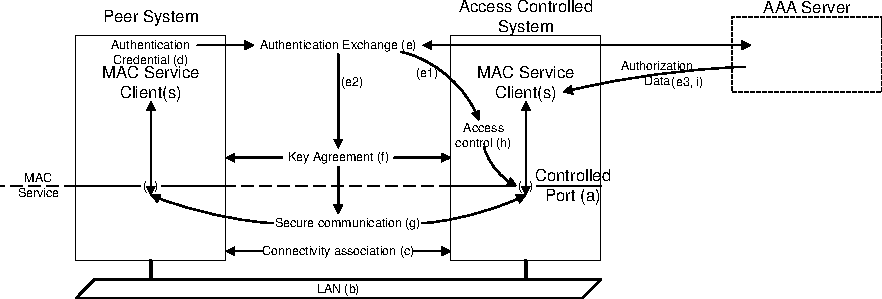
\includegraphics[width=1.0\linewidth]{8021x_fig_6_1_overview.pdf}
    \caption{Schematic overview of an 802.1X controlled Port with MACSec and an external AAA Server\cite{IEEE8021X}.}\label{fig:8021x_fig_6_1_overview}
\end{figure}

Figure \ref{fig:8021x_fig_6_1_overview} shows a high-level overview of an 802.1X enabled port with an external Authentication Server. The exchange of authentication credentials is done between the Peer and an Authenticator using the \ac{EAPOL} protocol and forwarded to an \ac{AAA} server. In the corresponding figure, RADIUS is chosen as the AAA protocol for practical reasons. The \ac{EAPOL} protocol is a Layer 2 protocol for the encapsulation of the \ac{EAP} authentication protocol. According to 802.1X, \ac{EAP} is not mandatory for mutual authentication, and \acp{PSK} may be used instead. Both methods result in a \ac{CAK} used as a root key for the MACSec key agreement protocol. In practice, \ac{EAP} is quite relevant in larger network installations since the flexibility of the protocol allows for a more scalable approach like X509 certificate-based authentication and authentication mechanism that use some kind of centralized directory.

\subsection{EAP and EAPOL}
The \acl{EAP}, as defined in RFC~3748\cite{rfc3748}, is a framework for network-based authentication protocols. As a framework, \ac{EAP} merely defines specific methods for authentication other than an MD5 challenge-response-based, an \ac{OTP}-based and a \ac{GTC}-based method. It is meant to be highly extensible regarding the authentication method, and a large number of methods were proposed since its initial release. While the \ac{EAP} standard itself defines no transport protocol, the 802.1X standard defines the \ac{EAPOL} transport protocol, which encapsulates \ac{EAP} messages in Ethernet frames with the corresponding Ethertype \texttt{0x888E}. \ac{EAPOL} defines four important \ac{EAPOL} \acp{PDU}:

\begin{enumerate}[itemsep=0pt]
    \item \textbf{\ac{EAPOL}-Start}\\
    An \ac{EAPOL}-Start message is sent either by the Supplicant or the Authenticator when the network link becomes available and can be periodically retransmitted until an answer from the other \ac{PAE} is received. This PDU is used to initiate the mutual authentication between the two \acp{PAE}.
    \item \textbf{\ac{EAPOL}-EAP}\\
    The \ac{EAPOL}-EAP \ac{PDU} is used to encapsulate \ac{EAP} messages as defined by RFC~3748. 
    \item \textbf{\ac{EAPOL}-Logoff}\\
    The \ac{EAPOL}-Logoff message is used when a \ac{PAE} wants to terminate the session. When MKA takes place, this type is ignored by the \acp{PAE} to mitigate DOS type attacks.
    \item \textbf{\ac{EAPOL}-MKA}\\
    The \ac{EAPOL}-MKA \ac{PDU} is used to transfer MK\acp{PDU} as defined by IEEE 802.1X. MK\acp{PDU} are used by the \ac{MKA} protocol to select a Key Server and derive cryptographic keys used by MACSec.
\end{enumerate}

EAP, and therefore EAPOL, works in a strict request-response fashion, where each EAP message needs to be acknowledged by the peer system before the next message is sent. This is done by two types of EAP messages: First, the Authenticator sends an \texttt{EAP-Request} messages of type \texttt{Identity} to the Peer. The Peer responses with a message of type \texttt{EAP-Response} that includes an identification string. The Authenticator sends the next message. It includes the requested \ac{EAP} method, which is either acknowledged by the Peer or responded to with a failure indicator if the requested method is not supported. After the Peer sends a successful response, a sequence of method-specific EAP messages is sent back and forth until the method results in a successful authentication or an unrecoverable error. As the last message, the Authenticator sends a status message with the Peer's authentication result.

\section{IEEE 802.1AE}
\begin{figure}[ht]
    \centering
    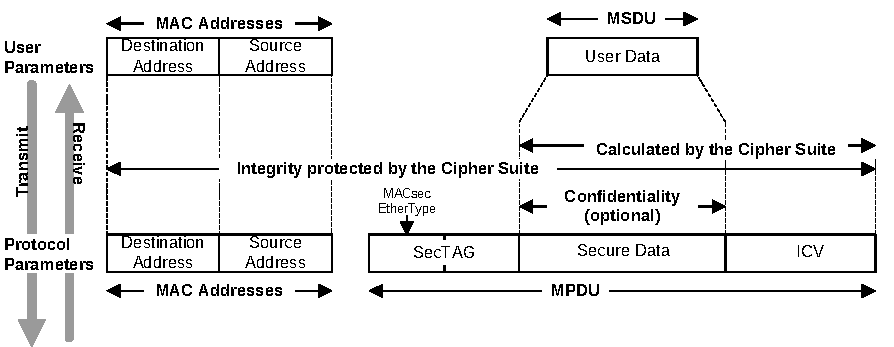
\includegraphics{8021ae_fig_8_1_macsec.pdf}
    \caption{The MACSec MPDU format\cite{IEEE8021X}}\label{fig:8021ae_fig_8_1_macsec.pdf}
\end{figure} 
The IEEE 802.1AE protocol suite focuses on ``connectionless user data confidentiality, frame data integrity, and data origin authenticity between security associations established by IEEE 802.1X''\cite{IEEE8021AE}. It describes the MACSec \ac{PDU} format and its encryption and integrity protection using the keys established by the MACSec key agreement protocol as described by IEEE 802.1X. MACSec defines a \ac{PDU} format, similar to Ethernet, to transmit frames in a local network that are integrity-protected and protected against eavesdropping through the use of symmetric cryptosystems. IEEE 802.1AE does not have any mandatory dependencies on IEEE 802.1X but is often used in conjunction. In such systems, IEEE 802.1X is used for mutual authentication and the initial key exchange of a single \ac{MSK}. The \ac{MSK} is shared between the Authenticator and the Peer entity. By using the MKA, both entities are now able to perform the \ac{MKA} protocol as an additional symmetric key-exchange protocol to exchange a \ac{LAN}-wide CAK, which is then used by MACSec to send encrypted and integrity-protect \acp{MPDU}. Figure~\ref{fig:8021ae_fig_8_1_macsec.pdf} provides a high-level overview of the \ac{MPDU} format. The MAC addresses are not a part of the \ac{MPDU} itself, but visualize how the format integrates into Ethernet frame-based networks. Instead of the usual Ethernet Ethertype, the Ethertype \texttt{0x885E} is transmitted as a part of the SecTAG format and signals that the following frame  is an \ac{MPDU}. The SecTAG further includes different protocol meta parameters, such as a MACSec internal version number, and whether confidentiality is used or only the integrity feature is used. The SECTag also includes an identifier of the \ac{CA} provided by 802.1X. The secure data field includes user data, which may be protected by symmetric encryption when confidentiality is used. The ICV field includes a cryptographically secured checksum to validate the integrity of the frame. It includes all fields of the \ac{MPDU} as well as the source and destination MAC addresses to protect against spoofing attempts. 


\subsection{MACSec Key Hierarchy}
\begin{figure}[ht]
    \centering
    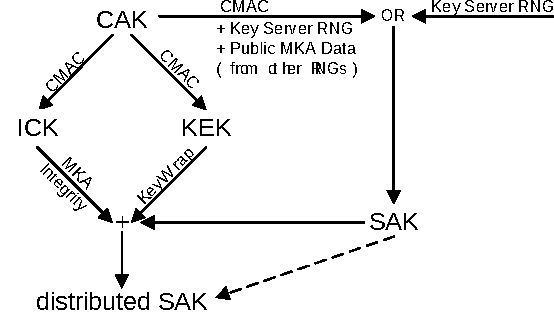
\includegraphics{8021x_fig_6_3_key_hierachy.pdf}
    \caption{Schematic overview of the MACSec Key Hierarchy\cite{IEEE8021X}}\label{fig:8021x_fig_6_3_overview}
\end{figure}

A shared symmetric key is needed on the Peer systems to provide confidentiality and integrity protection. This key is either a pre-shared secret or results from the authentication. Usually, MACSec requires an EAP method that supports the secure exchange of a 32-byte \ac{MSK} to the client. Figure~\ref{fig:8021x_fig_6_3_overview} shows an overview of the MACSec key hierarchy. The \ac{CAK} serves as a root key, which is not directly used for cryptographic purposes and is either derived from the EAP negotiated \ac{MSK} or from a static pre-shared key. Two further keys, the \ac{ICK} and the \ac{KEK}, are both derived from the \ac{CAK} using a \ac{KDF}. The \ac{ICK} is used to prove possession of the \ac{CAK} and for integrity protection of \acp{PDU}.

The \ac{SAK} is transferred to all members in a \ac{CA} and used for the actual encryption of \acp{PDU} by MACSec. The \ac{SAK} is generated and assigned to members of a \ac{CA} by a Key Server, which is elected by the members of the \ac{CA} using \ac{MKA}. In the case of a pairwise \ac{CAK} directly derived through \ac{EAP}, the role of the Key Server is always fulfilled by the Authenticator. For keys derive through any other method, the Key Server is selected by sending a ``Key Server Priority'' in each MK\ac{PDU}. Participants select the Key Server with the highest priority value. In case of a tie, the Key Server with the highest SCI value is chosen. The SCI value is a combination of the Key Servers MAC address and a numeric port identifier. Multiple Key Servers can generate a group \ac{CAK} to secure the system against the breach of a single \ac{CAK}. To generate the \ac{SAK}, either a strong random number generator on the Key Server or a \ac{KDF} can be used. In the case of distributed \acp{CAK}, each Key Server needs to generate the distributed \ac{CAK} by using a strong random number generator. To preserve the confidentiality of previously transmitted MKA frames, each distributed \ac{CAK} should be independent of any previous generated \ac{CAK} when a new participant joins the \ac{CA}\cite{IEEE8021X}.

\section{Classical Cryptography}


In the following chapters a bi-directional communication between two participants Alice \((A)\) and Bob \((B)\) is assumed. Participants use a cryptographic function \(f_e\) to transfer a cleartext message \(m\) to a ciphertext message \(c\) using a key \(k_e\) and another cryptographic function \(f_d\) to transfer the ciphertext \(c\) back into the cleartext \(m\) using a decryption key \(k_d\). Therefore, \(f_d(f_e(m,k_e),k_d) = m\). In the case of a symmetric cryptosystems, \(k_d = k_e\) holds.

\subsection{Asymmetric Cryptography}

In asymmetric cryptography, the cryptographic key of a participant consists of a private and a public part. The private part of the key is kept secret while the public part is published. To encrypt a message, Alice can use Bob's public key \(B_{k_{pub}}\) to generate a ciphertext. Decrypting the ciphertext is only possible in possession of Bob's private key \(B_{k_{priv}}\). Some digital signature schemes also use asymmetric primitives to provide authentication and integrity protection of the data. To provide a signature of the data, usually, a scheme involving cryptographic hash functions is used. For these schemes, Bob uses his private key to encrypt a hash value of the data. Alice can now use Bob's public key to decrypt the hash sent by Bob and compare it with a hash of the received data. If both hashes are equal, Alice knows with high probability that the hash was generated by the owner of the corresponding private key (e.~g., Bob) and the data were not tempered.

\begin{table}[t]
    \centering
    \caption{Overview of asymmetric key exchange and encryption schemes}

        \begin{tabular}{ l l c }
         \hline
         \textbf{Scheme} & \textbf{Related Problem} \\ 
         \hline
         \ac{RSA} &  Integer Factorization\\  
         Rabin &  Integer Factorization\\  
         \ac{DH} & Discrete Logarithm\\
         Elgamal & Discrete Logarithm \\
         \ac{ECDH} & Discrete Logarithm \\
         \ac{ECDSA} & Discrete Logarithm\\
         \ac{DSA} & Discrete Logarithm \\
    
        \end{tabular}
        \label{table:asymmetric_crypto_schemes}
\end{table}
    
Modern asymmetric (or public-key) crypto schemes rely on the computational complexity to invert certain mathematical functions. Inverting a function is referred to as the computational problem of the underlying cryptosystem, and strong crypto schemes are based on problems that are believed to be intractable. In this context, intractable means that no algorithm exists which can perform this inversion in at least polynomial time. Table~\ref{table:asymmetric_crypto_schemes} shows an overview of modern asymmetric cryptosystems and their underlying problem. It is easy to see that all listed cryptosystems relying on two important primitives. First, the problem of integer factorization, which depends on the complexity of calculating the integer prime factors of a large product \(N\). In RSA, \(N\) and an encryption exponent \(e\) are parts of the public key and therefore available to an attacker. By calculating \(c = m^e \mod N\), Alice can now transform any message into ciphertext. The ciphertext can be converted back into the message with the decryption exponent \(d\), by calculating \(m = c^d \mod N\). To calculate the private key \(d\), an attacker needs to know at least one of the two prime numbers. The second prime can easily be computed by \(x = N/p\). Since the only way to obtain the primes is to factorize the public available parameter \(N\), the cryptosystem's strength depends on the hardness of performing the algorithmic calculation of the (prime-)factorization in a cyclic field.

Another rather important primitive is called the discrete logarithm problem. This problem consists of finding the discrete logarithm \(x\) in a cyclic group \(p\) for \(b^x = a \bmod p \) where \(a\),  \(b\) and \(p\) denote large constants and \(p\) is prime. Instead of a encryption scheme, \ac{DLP}-based schemes like \ac{DH}-based variants, provide the notion of a key exchange protocol, rather than a encryption protocol. Instead of using a static public key for encryption, Alice and Bob are able to calculate a shared secret on-the-fly, using the public available generator \(g\) and a large prime \(p\). For this purpose Alice and Bob can locally compute \(g^a = A\) and \(g^b = B\) for large random numbers \(a\) and \(b\). Now both can exchange \(A\) and \(B\) and calculate \(A^b = C\) and  \(B^a = C\). This holds, because \(A^b = (g^a)^b = (g^b)^a = B^a\). The prime number \(p\) is used to perform all calculation in the cyclic group \(mod p\). An adversary only knows the prime \(p\), the generator \(g\) and both \(A\) and \(B\). To calculate the shared secret \(C\), an adversary need to know either \(a\) or \(b\), which can be found by calculating the discrete logarithm of either \(A\) or \(B\)


Alternatively to the definition of the discrete logarithm problem in finite fields like cyclic groups, a variant defined over elliptic curves is commonly used. An elliptic curve is defined over every point in a finite (Galois) field \(\mathbb{F}_q\) by the function \(E: y^2 = x^3 + ax +b\) with \(a,b \in k \) and \(4a^3 +27b^2 \neq 0\) together with the point of infinity \(\mathcal{O} = (0,1,0)\). The addition of two points and scalar multiplication on that curve is defined, which means that the results of the operations are also located on that curve, with \(\mathcal{O}\) as the neutral element. It is known that the exact definition of these operations, together with the elliptic curve, forms an abelian group. It is now possible to build a key exchange protocol on top of this structure analogous to the original \ac{DH} key exchange protocol by replacing the operations of modular exponentiation in a cyclic group with scalar multiplications and additions on the curve. A benefit of using elliptic curves over classical Diffie-Hellman is that the computational complexity of calculating the discrete logarithm problem on an elliptic curve grows linear instead of logarithmic growth in the classical variant. This allows the same security guarantees by using much smaller key sizes. Further, this allows the implementation of ephemeral \ac{DH} protocols that use a short-lived key, valid only for a single session, and therefore provides the cryptographically desirable notion of forward-secrecy.

As for today, all known algorithms that can solve these problems need at least subexponential time for a valid solution and breaking these schemes, therefore, is impractical, given sufficiently large problem space.

\subsubsection{\texorpdfstring{\acs{KEM}}{KEM} and \texorpdfstring{\acs{KEX}}{KEX}}
Two important terms that need further definition are \ac{KEX} and \ac{KEM}. Both are sometimes ambiguously used in literature. A \ac{KEX} is a protocol that allows Alice and Bob to agree on a shared cryptographic key by exchanging public, non-encrypted messages. An attacker is not able to retrieve the shared secret by intercepting these messages, while Alice and Bob can compute a shared key depending on some secret information in combination with the exchanged messages. An example of a \ac{KEX} is the \ac{DH} key exchange. A \ac{KEM} is a cryptographic protocol that uses an asymmetric scheme to confidentiality transfer a randomly generated secret from Alice to Bob or vice-versa. The public key of one party is used to encrypt the key, which then can be sent over a public channel to be decrypted by the party that possesses the corresponding private key. Both notions are tightly coupled and result in the mutual agreement on a single shared key, which can be used for further symmetric encryption.

\subsubsection{\texorpdfstring{\acf{PFS}}{PFS}}

In classical key exchanges like \ac{RSA}, a single long-term key pair is used for a large number of sessions. This results in a security risk. When the long-term key is compromised, it allows an attacker to decrypt already recorded key-exchanges subsequently. To avoid this problem, the notion of forward-secrecy or perfect forward-secrecy is employed. In a cryptosystem that supports forward-secrecy, an ephemeral key is used, which is only generated for a single session and not stored on any of the participants. A long-term key may still be required to sign the ephemeral key and avoid man-in-the-middle attacks, but this key needs to be independent of the exchanged keying material. Historically, ephemeral keys were no option since cryptosystems like \ac{RSA} requires too much overhead on key generation to use a distinct \ac{RSA} key pair for each session. With the development of more lightweight key exchange protocols like \ac{DH} and Elgamal, ephemeral key exchanges became more practical and are the de-facto standard and many modern cryptosystems like TLS.

\subsection{Symmetric Cryptography}

Unlike in asymmetric schemes, symmetric cryptosystems require Alice and Bob to use the same key for de- and encrypting a message. Applying the key to any plaintext yields the corresponding ciphertext. Applying the same key on the ciphertext again transfers the message back into the original plaintext. Two common distinctions for symmetric crypto schemes are whether the scheme is a so-called block or stream cipher. Stream ciphers are applied on a constant stream of bits, where block ciphers only encrypt blocks of a certain length and therefore may rely on some sort of padding of the small messages to match the block size. A common benefit of symmetric schemes is the performance that can be magnitudes of orders faster as with asymmetric schemes. Therefore cryptosystems like TLS often rely on asymmetric schemes solely to bootstrap a symmetric key between the participants, which is then used to encrypt the actual messages. A typical example of a secure and straightforward implementation of a symmetric cipher is \acl{OTP}. A simple \ac{OTP} implementation uses the XOR function and a pseudo-random number generator, seeded by the symmetric key, to provide a constant stream of keying material. The best-known attacks on such schemes are brute force type of attacks, where the attacker tries to guess the correct key. The security of such schemes, therefore, directly depends on the size of the keyspace.

\section{Post Quantum Cryptography}

With the rise of new quantum computing algorithms like Shor's and Grover's algorithm and the constant improvements of practical quantum computers, the field of \ac{PQC} gained a lot more relevance in recent years. This section will give an introduction to both algorithms and their application. Further, the ongoing \ac{NIST} standardization project for a suitable \ac{PQ} algorithm is discussed.


\subsection{Shor's Algorithm}

Instead of providing an algorithm that can be used to factorize arbitrary integers directly, Shor provides an algorithm that constructs an \ac{FFT} on a quantum computer in polynomial time. Shor uses this \ac{FFT} to calculate the order \(r\) of an element \(x\) in a multiplicative group \(G\) with the generator \(n\). This can be used by choosing a random element of this group and calculate the corresponding order. Afterwards, the greatest common divisor \(\gcd(x^{r/2},n)\) can be calculated which happens to be non trivial divisor of \(n\) if \(r\) is even and \(x^{r/2} \not\equiv -1 \pmod{n} \) holds. Due to the randomization, this yields a factor of \(n\) with a probability of \(\frac{1}{2}\) assuming two distinct prime factors for \(n\). Calculating the other prime factor is now a trivial division. For calculating the greatest common divisor, the Euclidean algorithm can be used, which can be implemented in polynomial time. The algorithm that builds the \ac{FFT} quantum gate also uses only polynomial time, resulting in an overall polynomial runtime for the factorization\cite{shor1999polynomial}.

Shor further shows in his work that the same algorithm for the quantum \ac{FFT} can be applied to solve the discrete logarithm problem as used in Diffie-Hellman based protocols. Since instances of \ac{ECDH} can be reduced to ordinary instances of the discrete logarithm problem in cyclic groups, this efficiently results in a polynomial-time algorithm for both the discrete logarithm problem for cyclic groups and elliptic curves.

\subsection{Grover's Algorithm}

In 1996 Grover published his work on a quantum algorithm that solves the problem of searching an element in an unsorted database with \(n\) elements in \(\bigo(\sqrt{n})\) steps. For any known classical algorithm, the time to find such an element would require \(\bigo(n)\) steps. It is commonly believed that no classical algorithm exists to solve this problem in less time. Bennett et al. proved in their work that the lower bound on any quantum computer is \(\bigo(2^{n/2})\)\cite{bennett1997strengths}, which makes Grover's algorithm within a constant time factor of an optimal solution. Grover uses a unitary matrix that implements a quantum oracle function \(f: \{0,1\}^* \to \{0,1\}\) on a superposition over all possible inputs. This oracle function is used to map the set of possible inputs to 1 if the input value would result in the required output. An example of such an oracle function would be a function that implements a hash function like SHA1 and would output 1 if the hash function's input is equal to the searched value. Grover proves in his work that the algorithm yields the desired element with a probability of \(\bigo(1)\)\cite{grover1996fast}. This has some implications for symmetric cryptosystems as described above since a brute force attack on the key can be interpreted as such a search, where the database is the complete keyspace of size \(2^n\) and the searched element is the symmetric key. Grover's algorithm, therefore, effectively weakens the security of the used cryptosystem by a quadratic factor.

\section{Post-Quantum Cryptography Standardization}
With respect to Shor's algorithm and the possibility of practical applications in the foreseeable future, the \ac{NIST} started a standardization project in December 2016 to decide on ``one or more additional public-key cryptographic algorithms to augment \ac{FIPS} 186-4, Digital Signature Standard (DSS), as well as special publications SP 800-56A Revision 2''\footurl{https://csrc.nist.gov/news/2016/public-key-post-quantum-cryptographic-algorithms}\footurl{https://csrc.nist.gov/publications/detail/fips/186/4/final}. The goal of this project is to provide a quantum-resistant, asymmetric crypto and signature scheme that can be used additionally or as an alternative to the currently specified algorithms that are affected by the work of Shor and the ongoing improvements of practical quantum computers. The initial call for submissions ended on November 30, 2017. The evaluation process is grouped into multiple rounds, where comments from the public and an ongoing discussion on the proposed algorithms are used to refine the selection of several acceptable cryptosystems for standardization. As for today, the project is currently in the third, and therefore final round of evaluation.


\begin{table}[ht]
    \centering
    \caption{Overview of the defined security level}
        \begin{tabular}{cll}
        \hline
         \textbf{Level} & \textbf{Primitive} & \textbf{Reference} \\
         \hline
         1 &  128-bit Block Cipher Key Search & AES128 \\
         2 &  256-bit Hash Function Collision & SHA256, SHA3-256 \\
         3 &  192-bit Block Cipher Key Search & AES92 \\
         4 &  384-bit Hash Function Collision & SHA384, SHA3-384 \\
         5 &  256-bit Block Cipher Key Search & AES256 \\
        \end{tabular}
        \label{table:nist_security_level}
    \end{table}


The call for submissions defines multiple so-called security levels. Each level is defined by a reference primitive and each submission is compared to one or more of these security levels. Submissions often define different parameter selection to match different security levels. The reference algorithms, as shown in Table~\ref{table:nist_security_level}, are well-studied crypto algorithms that can be used for ease of comparison with the submitted algorithms. Further, the following properties are defined as desirable:

\begin{enumerate}
    \setlength{\itemsep}{0pt}
    \item Perfect forward-secrecy
    \item Resistance to side-channel attacks
    \item Resistance to multi-key attacks
    \item Resistance to misuse
\end{enumerate}

All algorithms provide IND-CCA guarantees, while some algorithms also provide an IND-CPA compliant instance. The IND notation stands for ciphertext indistinguishability and is defined as an experiment where an attacker sends two chosen-plaintext messages of equal length to a challenger party with access to an encryption function \(E\) and a decryption function \(D\) seeded by an encryption key \(K_e\) and a decryption key \(K_d\). The challenger party decides to encrypt one of the two messages randomly, and the attacker tries to guess which of the chosen plaintext messages resulted in the returned ciphertext. The experiment further includes an encryption and decryption oracle, available to the attacker to encrypt and decrypt arbitrary messages under certain conditions.

\begin{itemize}
    \item \textbf{\ac{IND-CPA}} \\
    In this setting, the attacker is allowed a single iteration, i.~e., send two plaintext messages to the challenger and then have to decide which message results in the returned ciphertext. The attacker is further allowed to issue additional computations in polynomial time, including calls to the encryption oracle, before sending the plaintext and after receiving the ciphertext. These guarantees are needed to limit the attacker to computations in polynomial time.
    \item \textbf{\ac{IND-CCA}}
    In this setting, the attacker is further allowed to make arbitrary calls to a decryption oracle before sending the message to the challenger while keeping the restriction on a polynomial number of steps. This allows the attacker multiple iterations of calls to the encryption oracle and implies that multiple iterations do not weaken the cryptographic protocol.
    \item \textbf{\ac{IND-CCA2}}
    In this setting, the attacker is now additionally allowed to call the decryption oracle after he received to ciphertext from the challenger, with the only exception that the attacker is not allowed to send the received ciphertext itself to the oracle. This setting implies that an attacker has no additional advantage by using the decryption oracle after knowing the ciphertext that corresponds to one of the messages.  
\end{itemize}

Round 3 of the \ac{NIST} PQ project evaluates submissions under the guarantees provided by \ac{IND-CCA} with up to \(2^{64}\) queries to the oracle. This is useful for algorithms that depend on key re-usage and therefore require long-term security of the used keys. It is further allowed to submit additional cipher specifications that only provide \ac{IND-CPA} guarantees, with restrictions on the re-usage of a single key. This may be beneficial for schemes that have significant performance advantages under \ac{IND-CPA}.



\subsection{Public-key Encryption and Key-establishment Algorithms}

\begin{table}[ht]
    \centering
    \caption{\ac{NIST} Round 3 Candidates for asymmetric \ac{KEM} and \ac{KEX} algorithms. Candidates are either finalists or alternate candidates. Finalists are the preferred candidates by the \ac{NIST} and only minor changes are expected, while alternate candidates may be subject to more significant changes.}
    \begin{tabular}{llc}
            \hline
            \textbf{Background} & \textbf{Scheme} & \textbf{Finalist} \\
            \hline
            \multirow{3}{*}{Code-Based} 
            & BIKE & --- \\
            & Classic McEliece & \cmark \\
            & HQC & ---\\
            \hline
            \multirow{5}{*}{Lattice-Based} 
            & SABER & \cmark\\
            & CRYSTALS-KYBER & \cmark \\
            & NTRU & \cmark \\
            & NTRU Prime  & ---\\
            & FrodoKEM & --- \\
            \hline
            Isogeny-Based & SIKE & ---\\
            \hline
        \end{tabular}
    \label{table:nist_round_2_kem}
\end{table}

One part of the \ac{NIST} project is selecting one or more public key encryption or key encapsulation methods. Table~\ref{table:nist_round_2_kem} shows the currently discussed candidates, grouped by their mathematical foundation. In the remainder of this section, an introduction to the mathematical problems and their application for asymmetric cryptography is given.

\subsubsection{Lattice-based Key Exchange}

\begin{figure}[ht]
    \centering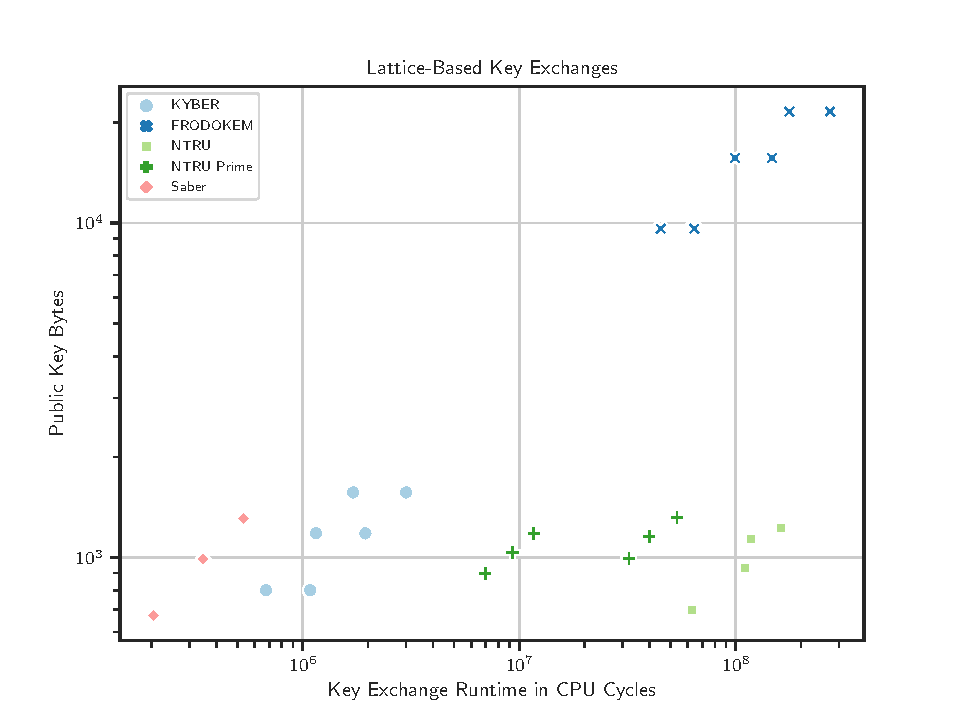
\includegraphics[width=1.0\linewidth]{plot_scatter_lattice_based_latency_pubkeysize.pdf}
    \caption{Overview of the current lattice-based Round 3 candidates of the \acs{NIST} \acs{PQ} standardization project. Only parameter selections with ING-CCA guarantees are shown. The x-axis shows the average latency for key generation, encapsulation and decapsulation of a shared secret in \acs{CPU} cycles on a logarithmic scale. The y-axis shows the public key size in bytes on a logarithmic scale. Benchmark results are part of eBACS\cite{eBACS}}\label{fig:lattice_level3_scatter}
\end{figure}

Lattice-based cryptosystems are based on the mathematical foundation of so-called lattices. A lattice is an n-dimensional geometric space with a periodical structure, described by a set of \(n\) linearly independent basis vectors \(b_1, \dots, b_n \in \mathbb{R}^n\), known as the basis \(B\) of a Lattice \(\mathcal{L}\). The lattice consists of points that are described by any linear combination of these vectors. The security of lattice-based systems depends on the hardness of multiple problems in these lattices\cite{micciancio2009lattice}.

\begin{enumerate}
    \setlength{\itemsep}{0pt}
    \item \ac{SVP} Find the shortest non-zero vector for a given basis \(B\)
    \item \ac{CVP} For a given basis \(B\) and a vector \(t\), find the lattice point closest to \(t\)
    \item \ac{SIVP} For a given basis \(B\) find a set set \(S\) of linearly independent vectors in \(\mathcal{L}(B)\) that minimize the quantity \(\Vert S \Vert = \max_i(\Vert s_i \Vert)\)
\end{enumerate}

Most lattice-based cryptosystems are not based on an exact solution to these problems but instead, use a variant where the solution needs to be within an approximation factor \(\gamma\). The best-known algorithms to solve these problems are running within polynomial time and give an approximation within an exponential factor. For an exact solution or a solution with an approximation factor within a polynomial factor, the best-known algorithms require exponential running time and space, making them impractical for a certain size for \(n\)\cite{micciancio2009lattice}. It is believed that there may be no algorithms that solve the \ac{SVP} in polynomial running time within a polynomial approximation factor. This hardness can be used to build cryptographic systems on top of these problems. Ajtai was the first that recognized the implication of lattice for cryptographic purposes by designing a one-way, collision-resistant hash function that can be reduced to the worst-case hardness of the \ac{SVP}\cite{ajtai1996generating}. In this context, worst-case hardness means that breaking these cryptosystems is at least as hard as breaking any \ac{SVP} instance within polynomial bounds, in polynomial time. Later, other cryptosystems were proposed on the foundation of Ajtai's work, including multiple public-key cryptosystems. As for now, lattice-based public-key cryptosystems seems to be a trade-off between practicability and proven security. Multiple proposed systems provide a desirable property of provable security by the cost of rather large key sizes. For example, a cryptosystem proposed by Ajtai and Dwork~\cite{ajtai1997public} with a worst-case hardness guarantee implies key sizes of serval gigabytes for lattices with a dimensional size up to ``serval hundreds''\cite{micciancio2009lattice}. Again, in this case, worst-case hardness means that breaking the system implies an efficient algorithm for any instance of the underlying lattice problem.

One instance of lattice-based public-key cryptosystems for which no such proof exists but which can be implemented efficiently and with practical key sizes is called NTRU. NTRU is a probabilistic cryptosystem, which means that it introduces some randomness into the encryption process and therefore results in many possible ciphertexts for a given plaintext\cite{hoffstein1998ntru}. The original description of NTRU is based on classical ring-based polynomial algebra but can also be given in the context of lattices. Another interesting class of lattice-based cryptosystems is based on the \ac{LWE} problem. The learning with error problem is a search problem which consists of finding a secret n-dimensional vector \(s \in Z_q^n\), given a polynomial number of vectors \(x_i \in Z_q^n\), where each vector is generated by sampling a random vector \(a_i \in Z_q^n \) and calculating the inner product \(b_i = \langle a_i, s \rangle \) and finally adding some noise by calculating \(x_i = b_i + r_i\) where \(r_i \in Z_q\) is sampled from a probability distribution. There is also an equivalent decision problem with the task to distinguish whether the set of noisy vectors is either completely randomly sampled from a uniform distribution or the result of the inner product combination, as shown above. It is shown that the search LWE problem can be reduced to a lattice-based approximate-\ac{SVP} and approximate-\ac{SIVP} by using a reduction algorithm that involves a quantum computer. That implies that an algorithm that solves these kinds of problems in polynomial time would provide a polynomial-time quantum algorithm that solves the approximate-\ac{SVP}.

On the other hand, this proof does not imply that the same hardness guarantees also holds for all classical algorithms. While cryptosystems based on the LWE problem provide better hardness guarantees that classical lattice-based cryptosystems like NTRU, the needed space to store the public key is still rather big compared to classical cryptosystems but still considered practical\cite{micciancio2009lattice}. A parameter selection of all Round 3 candidates with their latency and public key sizes is shown in Figure~\ref{fig:lattice_level3_scatter}. Except for \texttt{FrodoKEM}, all shown algorithms use public key sizes of a few KB. The main difference in Figure~\ref{fig:lattice_level3_scatter} are the \acs{CPU} cycles needed to generate a key pair and to encapsulate and decapsulate a shared secret. Depending on the algorithm, the differences are between a few orders of magnitude.

\subsubsection{Code-based Key Exchange}
\begin{figure}[ht]
    \centering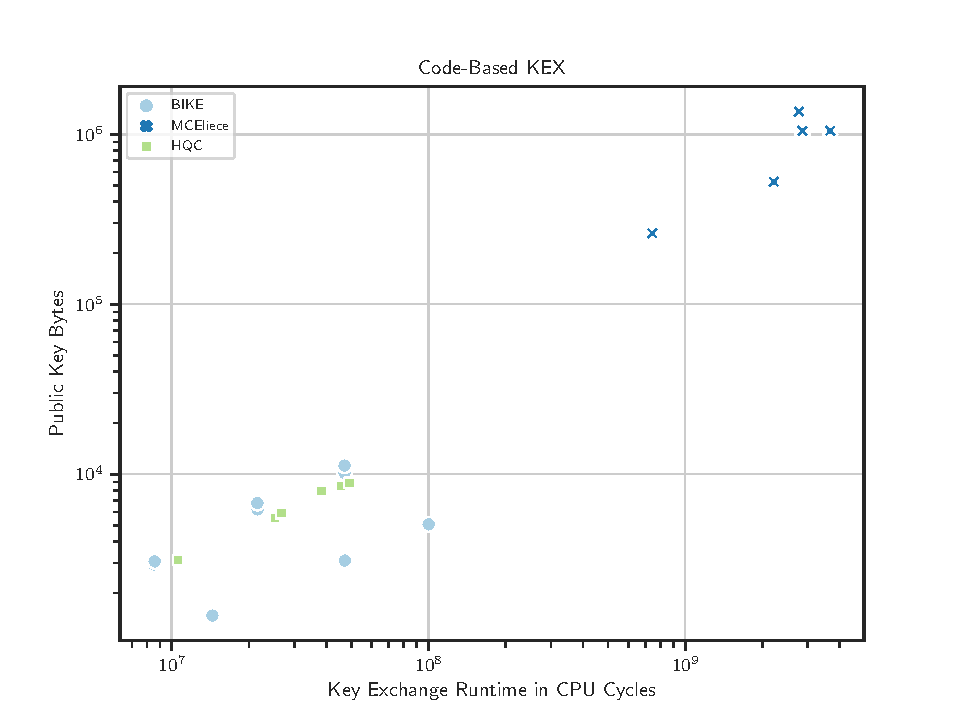
\includegraphics[width=1.0\linewidth]{plot_scatter_code_based_latency_pubkeysize.pdf}
    \caption{Overview of the current code-based Round 3 candidates of the \acs{NIST} \acs{PQ} standardization project. Only parameter selections with ING-CCA guarantees and \acs{NIST} security level 3 are shown. The axes are displayed on a logarithmic scale. The x-axis shows the average latency for key generation, encapsulation and decapsulation of a shared secret in \acs{CPU} cycles on a logarithmic scale. The y-axis shows the public key size in bytes on a logarithmic scale. Benchmark results are part of eBACS\cite{eBACS}}\label{fig:code_level3_scatter}
\end{figure}

Code-based cryptography is another promising candidate for \ac{PQC}. Cryptosystems in this category utilize the hardness of certain problems that arise from coding theory, which focuses on the design and algorithmic implementation of error detection and correction codes. The first proposal for a coding theory based public-key cryptosystem was designed by MCEliece in 1976. MCEliece uses a class of \ac{ECC} called general binary Goppa codes. The design relies on the fact that binary Goppa codes can be decoded efficiently, while no algorithm for general linear codes exists. McEliece uses this property to hide a Goppa code in a general linear code by randomly generating two matrices to transfer the matrix for the Goppa code into a matrix for a general linear code with the same distance and error rate as the original Goppa code. This matrix can be used as the public key, while the randomly generated matrices are used as the private key. A message can be encrypted by encoding the message into a code word in the general linear code and applying random errors to the resulting code word. To decrypt the message, an attacker needs to decode the general linear code and correct the random error, which is known to be NP-complete and for which no polynomial-time algorithm is believed to exists\cite{berlekamp1978inherent}. Alternatively, an attacker could restore the structure of the original generator matrix and decode the code word efficiently. While there are \ac{ECC} for which such an attack is possible, there is no such attack currently known for Goppa codes. With the knowledge of the two permutation matrices, it is computationally easy to transfer the message back into a binary Goppa code. By applying Peterson's algorithm, it is now possible to correct the random error and decode the code word back into the original message in polynomial time\cite{mceliece1978public}. Besides being released over 40 years ago, the original description by McEliece remains nearly unbroken in terms of that it provides nearly the same security level of \(2^{64}\) binary operations to break an instance of the cryptosystems with the parameters from the original paper. An attack first described by Canteaut and Sendrier\cite{canteaut1998cryptanalysis} and later refined by Bernstein et al.\cite{bernstein2008attacking} was able to reduce this value only to \(2^{60.55}\) while still using the parameters originally proposed by MCEliece. On the downside, the McEliece cryptosystem needs rather large public keys, ranging from multiple KB to a few MB. Multiple variants of Code-based cryptosystems were proposed in the past, using different types of codes or depending on different primitives to provide improvements in terms of the public key sizes. A parameter selection of all Round 3 candidates with their latency and public key sizes is shown in Figure~\ref{fig:code_level3_scatter}. Bike and the HQC scheme, which both rely on quasi-cyclic \acp{ECC}, are both able to provide better performance and key sizes than classic MCEliece.


\subsubsection{Isogeny-based Key Exchange}

\begin{figure}[ht]
    \centering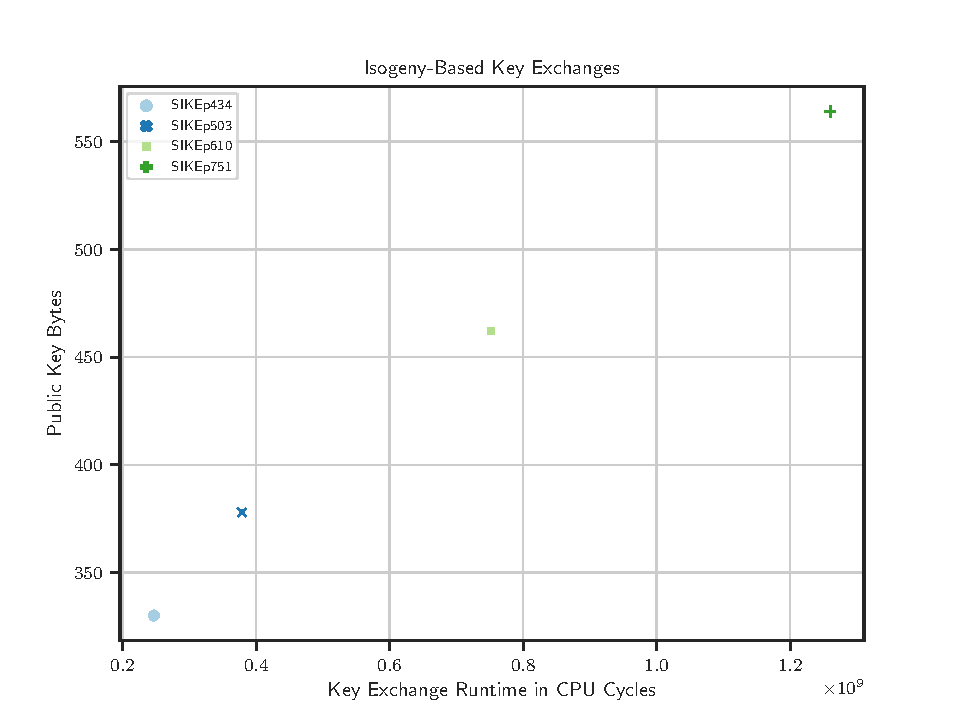
\includegraphics[width=1.0\linewidth]{plot_scatter_isogeny_based_latency_pubkeysize.pdf}
    \caption{Overview of the current implementations of the SIKE Round 3 candidates of the \acs{NIST} \acs{PQ} standardization project. All parameter selections that correspond to different security levels are shown. The x-axis shows the average latency for key generation, encapsulation and decapsulation of a shared secret in \acs{CPU} cycles. The y-axis shows the public key size in bytes. Benchmark results are part of eBACS\cite{eBACS}}\label{fig:sike_scatter}
\end{figure}

Instead of residing in completely new mathematical foundations for asymmetric cryptography, isogeny-based cryptographic protocols are located in the well-established field of \ac{ECC}. As for all problems which depend on the computational hardness of the discrete logarithm problem both, the cyclic group based \ac{DH} and \ac{EC}-based protocols are affected by Shor's algorithm and therefore are broken by a universal quantum computer. Isogeny-based \ac{EC} cryptography aims to solve this problem while still relying on elliptic curves, providing small public key sizes and allowing for ephemeral key exchanges. An isogeny \(\phi\) is a surjective mapping between two elliptic curves, such that that \(\phi\) is a group homomorphism. Another class of mappings between elliptic curves that is also a group homomorphism is called an isomorphism. An isomorphism is a bijective map between two elliptic curves. Two elliptic curves are isomorphic if and only if they have the same j-invariant. The j-invariant of an elliptic curve \(E \) is defined as \(j(E) = 1728 \frac{4a^3}{4a^3 +27b^2}\). Two j-invariant are isogenous if there exists an isogeny between the corresponding elliptic curves. It is now possible to view these isogenies as a graph. The vertices are a set of elliptic curves, described by their j-invariant and the edges represent the isogenies that map these j-invariants. These graphs are undirected since for every isogeny that maps \(E \to E'\); there is a corresponding isogeny that maps \(E' \to E\). Assuming an elliptic curve \(E\) defined over a finite field \(k\) with characteristics \(p\). For any prime \(l \neq p\) there exists \(l+1\) distinct isogenies of degree \(l\). This results in \(l+1\) edges for every vertex in the graph. These graphs are so-called expander graphs. Random walks on such expander graphs of a length close to the graph's diameter results in any vertex of the graph with a probability close to uniform. This random property can be used to build a cryptosystem on top of such graphs. In such a cryptosystem, both Alice and Bob generate two distinct isogeny graphs of degree \(l\), called \(l_A\) and \(l_B\) for a public curve \(E\). Now, both parties take a random walk in their respective graph of a certain length, depending on some large exponent \(e\). This results in two cyclic subgroups \(A, B \subset E\) with bases \(\langle P_A, Q_A \rangle\) and \(\langle P_B, Q_B \rangle\). Afterwards, both party publish \(A/ \langle E \rangle \) and \(B/ \langle E \rangle \), generated by their secret isogenies \(\alpha: E \to E/\langle A \rangle \) and \(\beta: E \to E/ \langle B \rangle\). For an attacker, it is a hard problem to calculate \(\alpha\) and \(\beta\) given \(E/ \langle A \rangle\) and \(E/ \langle B \rangle\), while there are efficient algorithms available to calculate the isogeny, given both curves. Additionally, Bob publish the values \(\beta(P_A)\) and \(\beta(Q_A)\). This allows Alice to generate \(\beta(A) E \to (E/\langle A \rangle)/ \langle B \rangle\) and vice-versa allows Bob to calculate \(\alpha(B) E \to (E/ \langle B \rangle )/A\). Since, \((E/ \langle B\rangle )/ \langle A \rangle\) and \((E/\langle A \rangle)/ \langle B \rangle\) are isomorphic, they share the same invariant which therefore can be used as a shared secret\cite{DBLP:journals/corr/abs-1711-04062}. Figure~\ref{fig:dh_dlog_isogeny} shows a simplified overview of the link between the key agreement in classical DH based protocols and the isogeny based variants. Both systems use an elliptic curve as a common base and communicate some public parameters. A combination of the private information, combined with the public parameters, results in a shared secret \(g^{ab}\) and \( E / \langle A, B \rangle\), respectively.

\begin{figure}[!ht]
    \centering
\begin{tikzpicture}[auto,node distance=1.3cm]
    \begin{scope}
        \matrix (m) [matrix of math nodes,
        row sep=4em,
        column sep=4em,
        minimum width=2em] {
        E                     & E / \langle A \rangle    \\
        E / \langle B \rangle & E / \langle A, B \rangle \\
        };
        \path[-stealth]
        (m-1-1) edge node [above] {$\phi_A$}  (m-1-2)
        (m-1-1) edge node [left]  {$\phi_B$}  (m-2-1)
        (m-2-1) edge node [below] {$\phi_A'$} (m-2-2)
        (m-1-2) edge node [right] {$\phi_B'$} (m-2-2);
    \end{scope}

    \begin{scope}[xshift=5cm]
        \matrix (m) [matrix of math nodes,
        row sep=4em,
        column sep=4em,
        minimum width=2em] {
        E                     & A    \\
        B &  g^{ab}\\
        };
        \path[-stealth]
        (m-1-1) edge node [above] {$g^a$}  (m-1-2)
        (m-1-1) edge node [left]  {$g^b$}  (m-2-1)
        (m-2-1) edge node [below] {$B^a$} (m-2-2)
        (m-1-2) edge node [right] {$A^b$} (m-2-2);
    \end{scope}
\end{tikzpicture}
\caption{High level overview of classical \ac{DH} on the right and isogeny based \ac{DH} on the left\cite{TikZ:for:Cryptographers}.}\label{fig:dh_dlog_isogeny}
\end{figure}

Due to their analogous behavior to related \ac{DH} type protocols, this class of algorithms is called \ac{SIDH}. The only instance of such key exchanges currently enlisted in the \ac{NIST} \ac{PQ} project is called SIKE. Figure~\ref{fig:sike_scatter} shows the currently proposed ciphers with different parameter selections to match certain security levels.

\subsection{Digital Signature Algorithms}

\begin{table}[ht]
    \centering
    \caption{\ac{NIST} Round 3 Candidates for \ac{DSS} algorithms}
    \begin{tabular}{llc}
            \hline
            \textbf{Background} & \textbf{Scheme} & \textbf{Finalist} \\
            \hline
            \multirow{2}{*}{Lattice-Based} 
            & CRYSTALS-DILITHIUM & \cmark\\
            & FALCON & \cmark \\
            \hline
            \multirow{2}{*}{Multivariate} 
                & GeMSS & \xmark\\
                & Rainbow & \cmark \\
            \hline
            Zero-Knowledge Proof & Picnic & \xmark \\
            \hline
            Hash-Based & SPHINCS+ & \xmark \\
            \hline
        \end{tabular}
    \label{table:nist_round_2_dss}
\end{table}

In addition to the mentioned public-key encryption and key-establishment algorithms, the \ac{NIST} \ac{PQ} project also focuses on a replacement for the currently used digital signature schemes. In practice, most of these schemes also rely on cryptographic protocols like \ac{RSA}, \ac{DH} or \ac{ECDH} and therefore are weakened by Shor's algorithm. Table~\ref{table:nist_round_2_dss} shows an overview of the currently discussed Round 3 candidates, grouped by their underlying mathematical primitives.

\subsubsection{Lattice-based Signatures}

\begin{figure}[!ht]
    \centering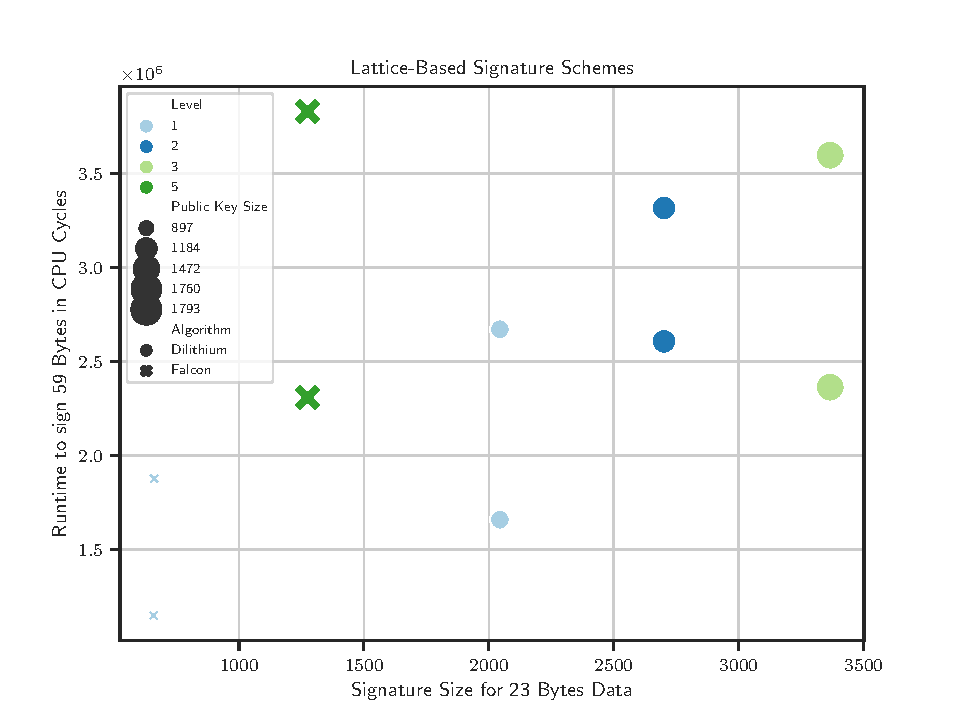
\includegraphics[width=1.0\linewidth]{plot_scatter_lattice_signlatency_signsize.pdf}
    \caption{Overview of the current implementations of lattice-based signature schemes in Round 3 of the \acs{NIST} \acs{PQ} standardization project. The y-axis shows the latency to sign a 59 Byte message in \acs{CPU} cycles. The x-axis shows the size of a signature for a 23 Byte message. The size of the markers reflects the relative size of the public keys. The color encodes the stated security level. Benchmark results are part of eBACS\cite{eBACS}}\label{fig:lattice_sign_scatter}
\end{figure}

Lattice-based schemes work on the foundation of lattice-based cryptography, as described in the last section. For \texttt{Dilithium}, a Fiat-Shamir construction is used to generate a non-interactive signature scheme from an interactive zero-knowledge proof. In general, such schemes work in a request-response fashion, where a challenger request proof from another party whether this party is the owner of a secret key, given the corresponding public key, without leaking information about the secret key. In an interactive setup, communication between both parties is required. However, there is a technique called Fiat–Shamir heuristics that allows implementing a non-interactive digital signature scheme by replacing the interactive request from the challenger with a cryptographic hash function over the message that needs to be signed. Initially, these schemes were designed for the \ac{RSA} cryptosystem\cite{fiat1986prove}. \texttt{Dilithium} is founded on a variation of this technique called Fiat-Shamir with aborts, which works for lattice-based systems. Since naive Fiat-Shamir-based implementations would leak information about the private key, assuming the signature is in a certain numerical range, this scheme allows the challenged party to abort a verification process if the resulting computation results in such a leak. The challenging party must restart the verification process until a valid signature is generated. The number of iterations depends on the probability of receiving a malicious random challenge that would result in a leak. In the original work by Lyubashevsky, the probability for a failure is a small constant of about \(2/3\). Therefore, only a small number of iterations is required until a successful signature is created. For one-time signatures, the same transformation can be applied. The signing party only needs to create valid signatures until a signature in the desired range is generated and then can continue to publish this signature, without the need of publishing the failed attempts\cite{10.1007/978-3-642-10366-7_35}.

In the case of \texttt{FALCON}, the signature scheme is based on one-way trapdoor permutation in lattices as described by Gentry, Peikert and Vaikuntanathan\cite{cryptoeprint:2007:432}. This construction uses a hash and sign scheme, where a message is hashed and encrypted by a lattice-based encryption function using the private key. The encryption function results in a vector in the lattice close to the hash value of the message. The distance between the pre-image of the message and the resulting vector can be used as a signature. To verify this signature, a challenger only needs to prove that the signature value is short (i.~e., close to the pre-image) and that the decrypted value is equal to the hashed value of the message.

The benefits of lattice-based schemes are the fast signature latencies and acceptable signature sizes. However, both come with the cost of rather large public keys. Figure~\ref{fig:lattice_sign_scatter} shows an overview of the different algorithms. \texttt{FALCON} places special focus on the combined sizes of the signatures and the public keys since both are usually needed to be transmitted in a certificate-based authentication setting. The plot shows that it achieves both goals compared to \texttt{Dilithium} and even outperforms all \texttt{Dilithium} designs in terms of signature size, even at the highest available security level.


\subsubsection{Multivariate-based Signatures}
\begin{figure}[ht]
    \centering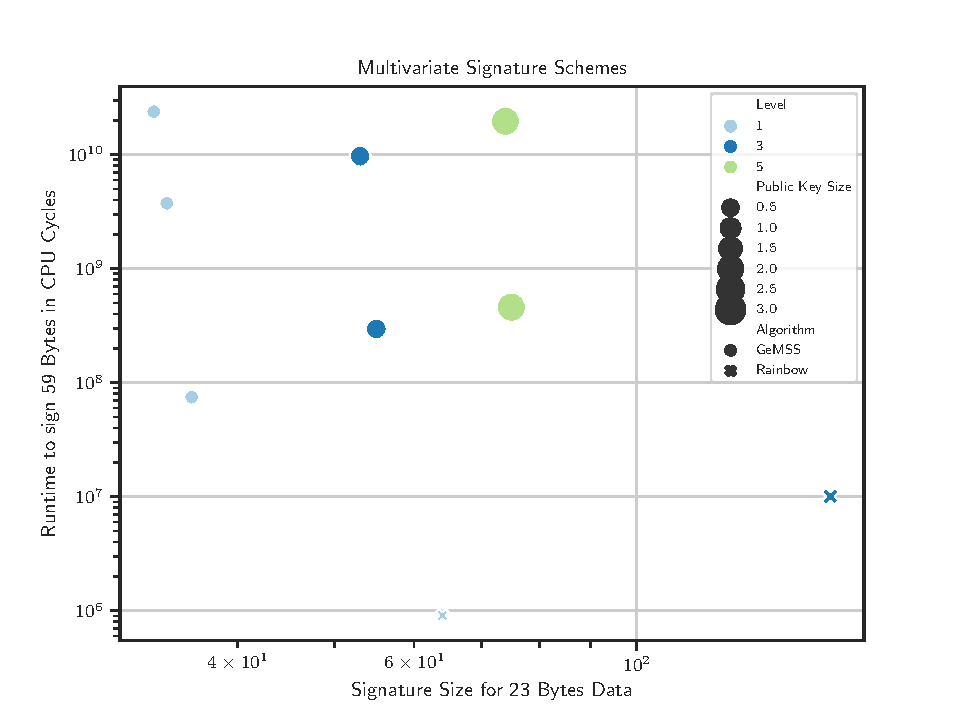
\includegraphics[width=1.0\linewidth]{plot_scatter_mv_signlatency_signsize.pdf}
    \caption{Overview of the current implementation of multivariate signature schemes in Round 3 of the \acs{NIST} \acs{PQ} standardization project. The y-axis shows the latency to sign a 59 Byte message in \acs{CPU} cycles on a logarithmic axis. The x-axis shows the size of a signature for a 23 Byte message. The size of the markers reflects the relative size of the public keys in KB. The color encodes the stated security level. Benchmark results are part of eBACS\cite{eBACS}}\label{fig:multivariate_sign_scatter}
\end{figure}

Multivariate signature schemes are based on the notion of multivariate cryptography. Multivariate crypto schemes are candidates for a \ac{PQ} key-exchange mechanism, and a few examples of such cryptosystems were part of the first round of the \ac{NIST} \ac{PQ} project. Since the \ac{NIST} had concerns regarding the full security of such systems, no multivariate key exchange advanced to the second round. However, they are still used as parts of multiple signature schemes. In general, multivariate cryptosystems are asymmetric cryptosystems that depend on the hardness of solving multivariate polynomials over a finite field, which is proven to be NP-complete. In a simplified design, based on a system called \ac{HFE}, the cryptosystem uses a finite field \(F_q\) of cardinality \(q\) and prime characteristics \(p\). Usually  \(p = 2\) is used. A polynomial \(f(x) = \sum_{i,j} \beta_{ij}x^{q^{\theta{ij}} + q^{\varphi{ij}}} + \sum_{k} a_{k} x^{q^{\epsilon_{k}}} + \mu \in F_{q^n}[x]\) for some random integers \(\varphi{ij}, \theta{ij}, \epsilon_{k} \geq 0 \), together with two affine transformation \(s, t: (F_q)^n \to (F_q)^n\) is chosen as the private key. A message \(x\) can be transformed to ciphertext by applying \(t(f(s(x))) = p_1(x_1, \dots, x_n) , \dots, p_n(x_1,\dots,x_n) \), where \(p_i\) are quadratic polynomials. Given \(f, t, s\) the polynomials \(p_i\) can be computed efficiently. The polynomials act as the public key and computing \(f, t, s\) given the public key corresponds to a hard problem\cite{patarin1996hidden}. Alternatives to this scheme are the  ``balanced oil and vinegar'' and the ``unbalanced oil and vinegar'' schemes. In balanced oil and vinegar systems, the secret key consists of a set of \(n\) equations that satisfy a certain structure. Each equation consists of secret coefficients, a number of \(n\) oil variables and a number of \(v\) vinegar variables. It is important that the equation does not compute a product of oil and vinegar variables, i.~e., the variables are not ``mixed''. For computing a valid signature, the vinegar variables are chosen randomly, and the oil variables are computed by a gaussian reduction. Both can be done efficiently in practice. The resulting signature can be verified using the public key, a matrix consisting of \(n\) equations that are generated by an affine transformation of the private key. In \ac{HFE} and oil and vinegar schemes, the signatures are valid if all equations in the public key are satisfied by the signature. For balanced systems \(n = v\) holds. However, there is a known attack when the number of oil variables is equal or within a small difference to the number of vinegar variables that allow an attacker to forge arbitrary signatures. \cite{kipnis1998cryptanalysis}\cite{kipnis1999unbalanced} This type of attack can be mitigated by unbalanced systems where \(v >> n\). The authors of \cite{kipnis1999unbalanced} showed that the attack is not applicable for \(v > 2n\) and propose a system with \(v \simeq \frac{n^2}{2} \). Furthermore, they described an algorithm that can efficiently break unbalanced schemes with \(v \geq n^2 \). Rainbow is a signature scheme that uses an unbalanced oil and vinegar construction. A benefit of using such schemes is that they can be implemented very efficiently in practice and provide small signature sizes. Figure~\ref{fig:multivariate_sign_scatter} shows a comparison of different signature schemes build on top of multivariate cryptosystems with respect to signature sizes and latencies. In a system based on the QUARTZ signature scheme, called GeMSS, a combination of the \ac{HFE} cryptosystem and so-called minus and vinegar modifiers are used to build a digital signature scheme. The minus modifier reduces the number of polynomials from the \ac{HFE} system that are published, and the vinegar modifier adds additional vinegar variables to the \ac{HFE} function \(f\). Both steps aim to add additional security to the classical \ac{HFE} notion\cite{patarin2001quartz}.

\subsubsection{Hash-based Signatures}


\begin{figure}[!ht]
    \centering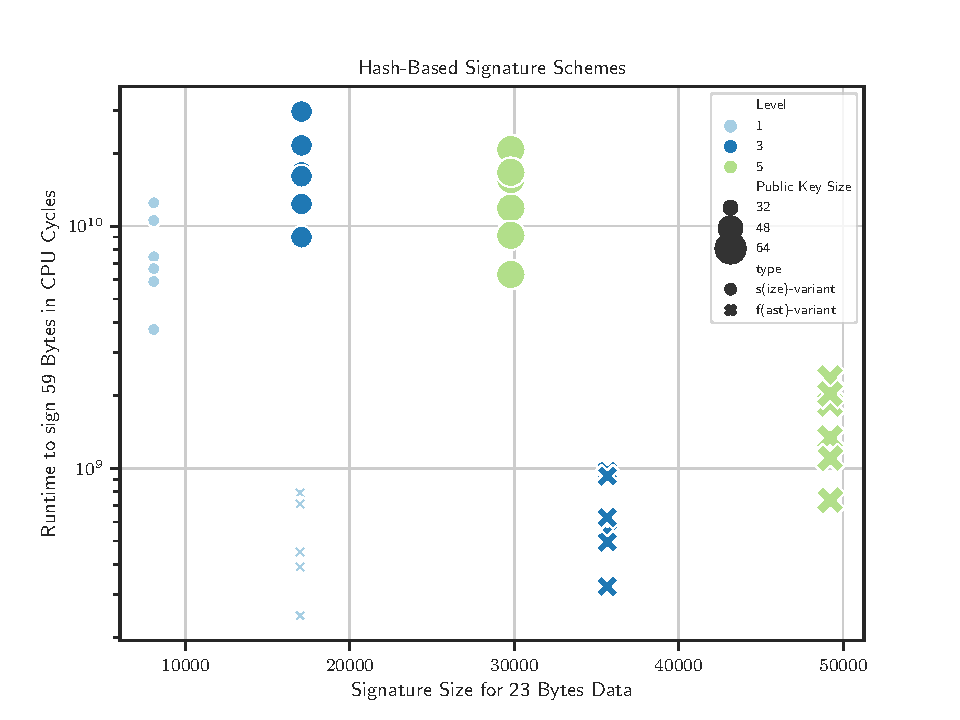
\includegraphics[width=1.0\linewidth]{plot_scatter_hash_based_signlatency_signsize.pdf}
    \caption{Overview of the current implementation of hash-based signature schemes in Round 3 of the \acs{NIST} \acs{PQ} standardization project. All security level 3 implementations are shown. The y-axis shows the latency to sign a 59 Byte message in \acs{CPU} cycles on a logarithmic axis. The x-axis shows the size of a signature for a 23 Byte message. Benchmark results are part of eBACS\cite{eBACS}}\label{fig:hash_sign_scatter}
\end{figure}

Instead of relying on a combination of asymmetric cryptography and cryptographic hash functions, hash-based signatures rely on the security of cryptographic hash functions only. The first construction that uses a hash-based approach was introduced by Lamport in 1979\cite{lamport1979constructing}. In his work, Lamport uses a one-way hash function \(F: \{0,1\}^* \to \{0,1\}^n\), for a fixed value \(n = 2^m\). The security of the system depends on the size of n and is typically in the range of \([128,512]\). First, Alice needs to compute \(n\) key pairs, where each element is a \(n\) bit long randomly generated number. The resulting set of numbers 
\(sk = (\{0,1\}^n)_{0,0}, (\{0,0\}^n)_{0,1}, (\{0,1\}^n)_{1,0}, (\{0,0\}^n)_{1,1}, \dots, (\{0,1\}^n)_{n,0}, (\{0,0\}^n)_{n,1}\) is used as the secret key. The public key consists of the \(n\) bit long hash value for each element \(pk = \{F(sk_i) \vert \forall i \le n \}\). To sign a single message \(m = \{0,1\}^n\), Alice signs each bit \(m_i\) individually by publishing the corresponding pair of the secret key \(x_{i,m_i}\). Bob can now verify the signature by calculating the hash value of each signature bit and compare it to the corresponding hash in Alice's public key. Since this method leaks parts of the secret key, it is obvious that using a single key pair for multiple signatures would allow an attacker to forge arbitrary signatures. Therefore Lamport's original scheme is a one-time signature scheme, meaning that every key pair can only be used to sign a single message. A further downside of this scheme is the rather large key sizes of \(2n^2\). As an alternative to this one-time scheme, multiple many-time schemes were proposed, allowing a single public key for more than a single application up to a fixed number of iterations. These schemes often use binary Merkle hash-trees as a compact data structure with a trade-off in terms of computational complexity. A Merkle tree is built in a bottom-up approach with a fixed number of leaves \(N=2^n\). In a Lamport like signature scheme, each leaf corresponds to a public-private-key pair \((sk_i, pk_i) \) as described above. The root of the hash tree is the newly published public key \(pk\). To sign a single message Alice now needs to publish a valid signature as a result of one \((sk_i,pk_i)\) key pair together with the corresponding one-time public key \(pk_i\) and the values for all \(n\) adjacent nodes that are included in the path from the root to the leaf. Bob can now validate the signature by reconstructing the path in the Merkle tree, using the underlying hash function and the signature, and comparing the result to the public key (i.~e. the root of the tree). The one-time signature leaves are usually used in a specific order from the leftmost to the rightmost leaf, which results in a total of \(N\) possible signatures. The size of the public key is decreased to a single hash value, while the size of the signatures is increased by a constant factor. A downside of this method is the fact that the whole tree needs to be computed upon key generation due to the bottom-up approach. this makes key generation and signature time exponential with respect to the height of the tree (and, therefore, the number of messages that can be signed). Further, this scheme reintroduces some kind of state into the signature process by requiring the signer to use an incrementing key-pair every time a message was signed. A stateless alternative to the data structure was proposed by Goldreich. Instead of a bottom-up tree approach, a top-down certificate tree is used. In this construction, the nodes of the binary tree use hash-based one-time signatures to sign both child nodes. The leaves of the tree correspond to one-time hash-based signatures to sign the actual messages. The secret key acts as a seed to a pseudo-random function to generate the tree ad-hoc. To ensure a single key pair is used only a single time, Goldreich proposed two methods. First, a \(n\) bit hash of the message is used as the index for a tree with height \(n\). This method ensures that a key pair is only used once as long as there is no collision in the used hash function. A downside of this scheme is the need for rather large signatures since the size of a single signature is cubic with respect to the size of the tree. An alternative approach is to select the index of the used leaf randomly. This allowed smaller tree sizes with a certain, negligible probability for key re-usage\cite{bernstein2015sphincs}. Currently, only a single instance of hash-based signature is a candidate for Round 3 of the \ac{NIST} \ac{PQ} project. SPHINCS+ is based on SPHINCS and uses a Goldreich construction with a so-called, few-times signature scheme and a hypertree construction to reduce the sizes of the signatures drastically by increasing the time to sign a single message. Contrary to one-time hash-based signatures, few-time hash-based signatures allow reusing a single public-private key-pair a limited amount of time. In the original design of SPHINCS, the usage of few-time signatures allowed to decrease the height of the tree from \(256\) to \(60\) while maintaining the same post-quantum security guarantees\cite{bernstein2015sphincs}. The usage of a hypertree model for the Goldreich tree allowed a further reduction of the signatures sized by increasing signature time exponentially with respect to the number of layers used in the hypertree. Figure~\ref{fig:hash_sign_scatter} shows an overview of the different SPHINCS+ implementations. All algorithms are implemented as an s-variant (size) and an f-variant (fast), optimized either for signature sizes or signature time.

\subsubsection{Zero-Knowledge-Proofs on Arbitrary Circuits}

\begin{figure}[!ht]
    \centering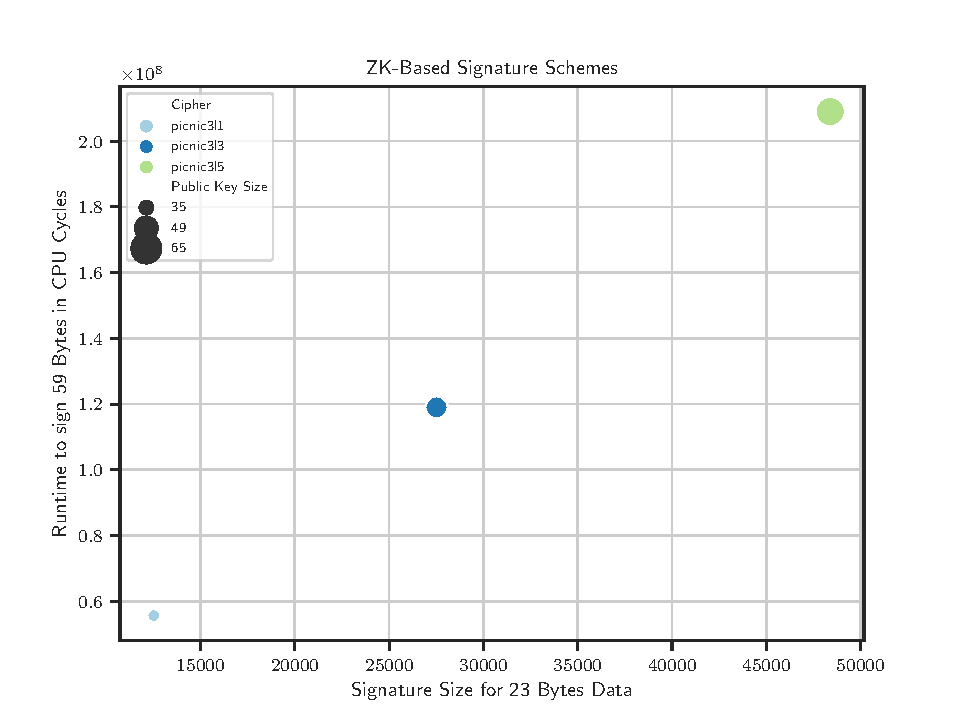
\includegraphics[width=1.0\linewidth]{plot_scatter_zk_signlatency_signsize.pdf}
    \caption{Overview of the current implementation of ZK-based signature schemes in Round 3 of the \acs{NIST} \acs{PQ} standardization project. All security level 3 implementations are shown. The y-axis shows the latency to sign a 59 Byte message in \acs{CPU} cycles on a logarithmic axis. The x-axis shows the size of a signature for a 23 Byte message. Benchmark results are part of eBACS\cite{eBACS}}\label{fig:zk_sign_scatter}
\end{figure}

As in hash-based signature schemes, ZK-proofs on arbitrary circuits based schemes use symmetric, polynomial-time computable primitives such as the SHA or AES function families to prove to a challenging party \(V\) that the proving party \(P\) knows some secret \(x\) without revealing information about the secret itself. In a system called ZKBoo, this works by interpreting the symmetric primitive as a binary relation \(R \subset \{0,1\}^* \times \{0,1\}^*\), where the result of the computation is a relation of the inputs to the output of the symmetric primitive e.~g. \( R = \{(x,y) \vert y = SHA(x)\}\). The language L is the set of \(x\) variables for a given \(y\) that results in a ``yes'' answer (e.~g. \(R(x,y) = 1\))\cite{giacomelli2016zkboo}. When looking at SHA1 as an example, the language L is the set of all tuples \((x,y)\) that result in some hash value \(y\) for all possible inputs \(x\). In this protocol, the proofer \(P\) wants to convince a verifier \(V\) that he knows an instance \(l \in L\), without revealing the associated \(x\). In other words, the proofer wants to convince the verifier that he knows an input to the symmetric primitive that results in the publicly available result of the computation. ZKBoo uses a so-called \ac{MPC} protocol. In this protocol, a set of \(n\) participants know the used symmetric primitive and have access to a secret value \(x_i\). The goal of each player is to compute \(f(x) = y\) with \(x = (x_1,\dots,x_n)\) without revealing \(x_i\). Players can communicate over secure point-to-point channels. Each player computes a view that consists of the secret value concatenated with random data and its history of past communication. After multiple rounds, the output \(y\) can be computed from any view without gaining any information about the private value from some other player. The protocol is said to be robust if it is possible to produce the correct value \(y\) for any view, even if another player tries to intentionally manipulate the calculation. The ZKBoo protocol uses a virtualized version of the \ac{MPC} protocol where each player is simulated by the prover. After the view of each player is computed, a so-called \(\Sigma\) protocol is used as a three-way interactive prove. In this \(\Sigma\) protocol, two out of the three views and all results of the \ac{MPC} protocol are sent to the verifying party, depending on an index randomly chosen by the verifier. The verifying party can now check if the computed outputs match the public value \(y\) and if the revealed views are consistent. In this context, consistency of the views means that the verifier can detect whether the proofer tries to prove a false statement. By only revealing a subset of the views, \(P\) can ensure that \(V\) is not able to calculate the secret value from the available data. This effectively creates a zero-knowledge prove of \(x\), based on a composition of a symmetric primitive \(f(x) = y \) used in the \ac{MPC} protocol. The used function divides the computation of the primitive into three branches. Each branch uses a share of its own input and the share of the neighboring input, effectively limiting the \ac{MPC} protocol to three parties\cite{giacomelli2016zkboo}. A primitive used in the \ac{NIST} \ac{PQ} project called Picnic extends the ZKBoo protocol to a protocol called ZKB++. Different optimizations used in the ZKB++ protocol allows for less than half of the size for a proof by keeping the computational costs the same\cite{cryptoeprint:2017:279}. Since the ZKB++ protocol is still interactive, the Picnic authors provide two ways to construct a non-interactive scheme based on the interactive variant. The first scheme, called Fish, uses a Fiat-Shamir transform, as explained in the last sections. The actual variant used for Picnic is based on an Unruh transformation. In \cite{unruh2012quantum}, Unruh provides a transformation for \(\Sigma\) zero-knowledge proof protocols in a quantum random oracle model and proves that it is secure in the presence of a quantum adversary, assuming the property of ``strict and special soundness''.


\section{Related Work}

Quantum-resistant cryptosystems have been researched since it became known that the security of currently used cryptosystems is degraded by quantum computers. The \ac{NIST} standardization project explicitly does not aim to select a single \ac{PQ} key exchange suitable for all applications but rather tries to select a few interesting primitives with different trade-offs between the key size or the performance of the algorithms. Therefore, additional work needs to be done to evaluate one or more suitable algorithms for certain use-cases. As a part of the QuaSiModO research project, such effort was already put into the design of a quantum resistance key exchange for the IKEv2 key exchange protocol\cite{exchangetowards}. Another notable project, called Open Quantum Safe focuses on ``prototyping quantum-resistant cryptography, which includes liboqs, a C library of quantum-resistant algorithms, and [the] integrations of liboqs into popular open-source applications and protocols, including the widely used OpenSSL library.''\cite{stebila2016post} A case-study that uses liboqs to implement post-quantum aware key exchange and authentication protocols in TLS and SSH is available\cite{crockett2019prototyping}.

Multiple \ac{IETF} Internet-Drafts propose a so-called hybrid key exchange method. In such hybrid key exchanges, classical algorithms are combined with quantum-resistant algorithms to provide the quantum resistance property of these newer algorithms while maintaining the guarantees of well researched classical algorithms. 

An Internet-Draft for TLS 1.2\cite{whyte-qsh-tls12-02} focuses on a hybrid mode handshake using NTRU for a quantum-safe cipher. The draft defines a new cipher suite called TLS\_QSH. Further, two extensions to the TLS protocol are defined to allow a custom state machine suited for the needs of a hybrid key exchange. Both extensions allow an additional quantum-safe key exchange in the TLS handshake before a classical key exchange takes place. A combination of both keys is used to generate a session key that is safe against classical attacks as well as a quantum adversary. The authentication and authenticity of the data in this scheme are only derived from a classical cipher suite, which allows a quantum adversary to break these guarantees. Internet-Draft \cite{schanck-tls-additional-keyshare-00} is a proposal that makes use of a TLS 1.3 feature, called ``\texttt{key\_share}'', which allows combining a session key from multiple shared secrets. By its original design, this feature is used to combine a key derived from a pre-shared secret with an ephemeral \ac{DH} key to achieve forward-secrecy for PSK based key exchanges or to allow a handshake to include multiple DH parameters. The document defines extensions to a set of TLS handshake messages that allows to include an additional non-\ac{DH} based key exchange in the \texttt{key\_share} extension. This additional secret may be generated by any quantum-safe key exchange mechanism and can be used as an input for a key derivation function to generate a quantum-safe session secret. IETF draft \cite{kiefer-tls-ecdhe-sidh-00} also makes use of the \texttt{key\_share} extension to additionally include an isogeny-based key exchange in the TLS handshake. Instead of defining a new extension, the draft makes use of the existing extension to transfer the additional \ac{SIDH} based key as an additional \texttt{key\_share} entry. \cite{whyte-qsh-tls13-06} works by defining new hybrid modes as possible TLS ciphers instead of interpreting the hybrid key exchange as two distinct ciphers. This way, the current TLS implementation can be used without major modification to the protocol. When a hybrid cipher is selected (e.\ g., \texttt{secp256r1}+\texttt{sikep503}), the \texttt{key\_share} entry variable-length field consists of a custom data structure that includes both key exchange parameters. If only a classical cipher is used (e.\ g., \texttt{secp256r1}), the \texttt{key\_share} entry is used as already defined by the TLS standard. This way, existing TLS implementation could be used in a backward-compatible manner. Since the new cipher type is unknown to non-quantum aware implementations, the cipher would not be selected in the negotiation process. The same approach is used in another internet-draft\cite{ietf-tls-hybrid-design-02}, which opposed to the other mentioned drafts, is still being actively maintained. The TLS implementation used in the liboqs OpenSSL integration is based on an earlier version of \cite{ietf-tls-hybrid-design-02}.

The security division of Google LLC also worked with hybrid modes in two experiments. In 2016, an implementation of the NewHope algorithm was used in addition to a regular elliptic curve key exchange for a small fraction of TLS 1.2 connections between a nightly build of the Chrome web browser and some Google domains\cite{cecpq1}. A second experiment, which uses the NTRU algorithm on top of an elliptic curve key exchange for TLS 1.3 connections, was launched in 2018\cite{cecpq2}.

A blog post by Cisco Systems, Inc., proposes using pre-shared keys in combination with symmetric cryptography to achieve quantum-resistant encryption for the MACSec protocol but does not further look into using \ac{EAP} for mutual authentication and defers the problem until TLS implements a \ac{PQ} key exchange method\cite{ciscopqmacsec}. A technical report by the \ac{ETSI} on quantum-safe \acp{VPN} partially focuses on a quantum-resistant MACSec implementation. In this report, the \ac{ETSI} also advises on using pre-shared keys and the use of symmetric cryptography. For quantum-resistant TLS-based authentication, the document refers to hybrid modes but does not make any further recommendations regarding cryptographic protocols or MACSec-specific parameters. 

\endinput

% ---------------------------------------------------------------
\backmatter % ab hier keine Nummerierung mehr
    \listoffigures
    \bibliographystyle{alphadin}
    \bibliography{./Bib/stud77}

\end{document}
